\documentclass{vkr}
\usepackage[english, russian]{babel} % переносы
\usepackage{graphicx} % для вставки картинок
\graphicspath{{images/}} % путь к изображениям
\usepackage[hidelinks]{hyperref}
\usepackage{float} % определяет метод H для рисунка с переносом на следующую страницу, ели не помещается
\usepackage{pdflscape}
\addto{\captionsrussian}{\renewcommand{\refname}{СПИСОК ИСПОЛЬЗОВАННЫХ ИСТОЧНИКОВ}}
\usepackage{xltabular} % для вставки таблиц
\usepackage{makecell}
\renewcommand\theadfont{} % шрифт в /thead
\usepackage{array} % для определения новых типов столбцов таблиц
\newcolumntype{T}{>{\centering\arraybackslash}X} % новый тип столбца T - автоматическая ширина столбца с выравниванием по центру
\newcolumntype{R}{>{\raggedleft\arraybackslash}X} % новый тип столбца R - автоматическая ширина столбца с выравниванием по правому краю
\newcolumntype{C}[1]{>{\centering\let\newline\\\arraybackslash\hspace{0pt}}m{#1}} % новый тип столбца C - фиксированная ширина столбца с выравниванием по центру
\newcolumntype{r}[1]{>{\raggedleft\arraybackslash}p{#1}} % новый тип столбца r - фиксированная ширина столбца с выравниванием по правому краю
\newcommand{\centrow}{\centering\arraybackslash} % командой \centrow можно центрировать одну ячейку (заголовок) в столбце типа X или p, оставив в оcтальных ячейках другой тип выравнивания
\newcommand{\finishhead}{\endhead\hline\endlastfoot}
\newcommand{\continuecaption}[1]{\caption*{#1}\\ \hline }
\usepackage{etoolbox}
\AtBeginEnvironment{xltabular}{\refstepcounter{tablecnt}} % подсчет таблиц xltabular, обычные таблицы подсчитываются в классе

\usepackage[tableposition=top]{caption} % подпись таблицы вверху
\captionsetup{strut=off}
\setlength{\intextsep}{0pt} % Vertical space above & below [h] floats
\setlength{\textfloatsep}{0pt} % Vertical space below (above) [t] ([b]) floats
\DeclareCaptionLabelFormat{gostfigure}{Рисунок #2} %подпись рисунка
\DeclareCaptionLabelFormat{gosttable}{Таблица #2} %подпись таблицы
\DeclareCaptionLabelSeparator{gost}{~--~} %разделитель в рисунках и таблицах
\captionsetup{labelsep=gost}
\captionsetup[figure]{aboveskip=10pt,belowskip=4mm,justification=centering,labelformat=gostfigure} % настройка подписи рисунка
\captionsetup[table]{font={stretch=1.41},skip=0pt,belowskip=0pt,aboveskip=8.5pt,singlelinecheck=off,labelformat=gosttable} % настройка подписи таблицы

\setlength{\LTpre}{8mm} % отступ сверху таблицы
\setlength{\LTpost}{6mm} % отступ снизу таблицы

\usepackage{enumitem}
\setlist{nolistsep,wide=\parindent,itemindent=*} % отступы вокруг списков, выравнивание с учетом разделителя

\usepackage{color} %% это для отображения цвета в коде
\usepackage{listings} %% листинги кода
\setmonofont[Scale=0.7]{Verdana} % моноширный шрифт для листинга

\definecolor{codegreen}{rgb}{0,0.6,0}
\definecolor{codegray}{rgb}{0.5,0.5,0.5}
\definecolor{codepurple}{rgb}{0.58,0,0.82}

\lstset{ %
language=C,                 % выбор языка для подсветки (здесь это С)
numbers=left,               % где поставить нумерацию строк (слева\справа)
numberstyle=\tiny,           % размер шрифта для номеров строк
stepnumber=1,                   % размер шага между двумя номерами строк
numbersep=5pt,                % как далеко отстоят номера строк от подсвечиваемого кода
commentstyle=\color{codegreen},
keywordstyle=\color{magenta},
numberstyle=\tiny\color{codegray},
stringstyle=\color{codepurple},
basicstyle=\linespread{0.95}\ttfamily,
backgroundcolor=\color{white}, % цвет фона подсветки - используем \usepackage{color}
showspaces=false,            % показывать или нет пробелы специальными отступами
showstringspaces=false,      % показывать или нет пробелы в строках
showtabs=false,             % показывать или нет табуляцию в строках
frame=single,              % рисовать рамку вокруг кода
tabsize=2,                 % размер табуляции по умолчанию равен 2 пробелам
captionpos=t,              % позиция заголовка вверху [t] или внизу [b] 
breaklines=true,           % автоматически переносить строки (да\нет)
breakatwhitespace=false, % переносить строки только если есть пробел
escapeinside={\%*}{*)}   % если нужно добавить комментарии в коде
}

\makeatletter % чтобы допускались русские комментарии в листингах
\lst@InputCatcodes
\def\lst@DefEC{%
 \lst@CCECUse \lst@ProcessLetter
  ^^80^^81^^82^^83^^84^^85^^86^^87^^88^^89^^8a^^8b^^8c^^8d^^8e^^8f%
  ^^90^^91^^92^^93^^94^^95^^96^^97^^98^^99^^9a^^9b^^9c^^9d^^9e^^9f%
  ^^a0^^a1^^a2^^a3^^a4^^a5^^a6^^a7^^a8^^a9^^aa^^ab^^ac^^ad^^ae^^af%
  ^^b0^^b1^^b2^^b3^^b4^^b5^^b6^^b7^^b8^^b9^^ba^^bb^^bc^^bd^^be^^bf%
  ^^c0^^c1^^c2^^c3^^c4^^c5^^c6^^c7^^c8^^c9^^ca^^cb^^cc^^cd^^ce^^cf%
  ^^d0^^d1^^d2^^d3^^d4^^d5^^d6^^d7^^d8^^d9^^da^^db^^dc^^dd^^de^^df%
  ^^e0^^e1^^e2^^e3^^e4^^e5^^e6^^e7^^e8^^e9^^ea^^eb^^ec^^ed^^ee^^ef%
  ^^f0^^f1^^f2^^f3^^f4^^f5^^f6^^f7^^f8^^f9^^fa^^fb^^fc^^fd^^fe^^ff%
  ^^^^20ac^^^^0153^^^^0152%
  % Basic Cyrillic alphabet coverage
  ^^^^0410^^^^0411^^^^0412^^^^0413^^^^0414^^^^0415^^^^0416^^^^0417%
  ^^^^0418^^^^0419^^^^041a^^^^041b^^^^041c^^^^041d^^^^041e^^^^041f%
  ^^^^0420^^^^0421^^^^0422^^^^0423^^^^0424^^^^0425^^^^0426^^^^0427%
  ^^^^0428^^^^0429^^^^042a^^^^042b^^^^042c^^^^042d^^^^042e^^^^042f%
  ^^^^0430^^^^0431^^^^0432^^^^0433^^^^0434^^^^0435^^^^0436^^^^0437%
  ^^^^0438^^^^0439^^^^043a^^^^043b^^^^043c^^^^043d^^^^043e^^^^043f%
  ^^^^0440^^^^0441^^^^0442^^^^0443^^^^0444^^^^0445^^^^0446^^^^0447%
  ^^^^0448^^^^0449^^^^044a^^^^044b^^^^044c^^^^044d^^^^044e^^^^044f%
  ^^^^0401^^^^0451%
  %%%
  ^^00}
\lst@RestoreCatcodes
\makeatother


% Режим шаблона (должен быть включен один из трех)
\ВКРtrue
%\Практикаtrue
%\Курсоваяtrue

\newcommand{\Дисциплина}{<<Проектирование и архитектура программных систем>>} % для курсовой
\newcommand{\КодСпециальности}{09.03.04} % Курсовая
\newcommand{\Специальность}{Программная инженерия} % Курсовая
\newcommand{\Тема}{Платформа для создания компьютерных изометрических ролевых игр} % ВКР Курсовая
\newcommand{\ТемаВтораяСтрока}{с заранее отрисованным двухмерным фоном и спрайтовыми персонажами}
\newcommand{\ГдеПроводитсяПрактика}{Юго-Западном государственном университете} % для практики
\newcommand{\РуководительПрактПредпр}{} % для практики
\newcommand{\ДолжнРуководительПрактПредпр}{директор} % для практики
\newcommand{\РуководительПрактУнивер}{Чаплыгин А. А.} % для практики
\newcommand{\ДолжнРуководительПрактУнивер}{к.т.н. доцент} % для практики
\newcommand{\Автор}{К. Н. Шевченко}
\newcommand{\АвторРод}{Шевченко К.Н.}
\newcommand{\АвторПолностьюРод}{Шевченко Клима Николаевича} % для практики
\newcommand{\Шифр}{20-06-0139}
\newcommand{\Курс}{4} % для практики
\newcommand{\Группа}{ПО-02б}
\newcommand{\Руководитель}{А. А. Чаплыгин} % для ВКР и курсовой
\newcommand{\Нормоконтроль}{А. А. Чаплыгин} % для ВКР
\newcommand{\ЗавКаф}{А. В. Малышев} % для ВКР
\newcommand{\ДатаПриказа}{«04» апреля 2024~г.} % для ВКР
\newcommand{\НомерПриказа}{1616-с} % для ВКР
\newcommand{\СрокПредоставления}{«25» июня 2024~г.} % для ВКР, курсового

\begin{document}
\maketitle
\ifПрактика{}\else{
   \newpage
\begin{center}
\large\textbf{Минобрнауки России}

\large\textbf{Юго-Западный государственный университет}
\vskip 1em
\normalsize{Кафедра программной инженерии}
\vskip 1em
\ifВКР{
        \begin{flushright}
        \begin{tabular}{p{.4\textwidth}}
        \centrow УТВЕРЖДАЮ: \\
        \centrow Заведующий кафедрой \\
        \hrulefill \\
        \setarstrut{\footnotesize}
        \centrow\footnotesize{(подпись, инициалы, фамилия)}\\
        \restorearstrut
        «\underline{\hspace{1cm}}»
        \underline{\hspace{3cm}}
        20\underline{\hspace{1cm}} г.\\
        \end{tabular}
        \end{flushright}
        }\fi
\end{center}
\vspace{1em}
  \begin{center}
  \large
\ifВКР{
ЗАДАНИЕ НА ВЫПУСКНУЮ КВАЛИФИКАЦИОННУЮ РАБОТУ
  ПО ПРОГРАММЕ БАКАЛАВРИАТА}
  \else
ЗАДАНИЕ НА КУРСОВУЮ РАБОТУ (ПРОЕКТ)
\fi
\normalsize
  \end{center}
\vspace{1em}
{\parindent0pt
  Студента \АвторРод, шифр\ \Шифр, группа \Группа
  
1. Тема «\Тема\ \ТемаВтораяСтрока»
\ifВКР{
утверждена приказом ректора ЮЗГУ от \ДатаПриказа\ № \НомерПриказа
}\fi.

2. Срок предоставления работы к защите \СрокПредоставления

3. Исходные данные для создания программной системы:

3.1. Перечень решаемых задач:}

\renewcommand\labelenumi{\theenumi)}

\begin{enumerate}
\item анализ существующих ролевых игр;
\item разработка концептуальной модели ролевых игр;
\item проектирование программной системы для создания ролевых игр;
\item реализация программной системы для создания ролевых игр;
\item тестирование разработанной системы.
\end{enumerate}

{\parindent0pt
  3.2. Входные данные и требуемые результаты для программы:}

\begin{enumerate}
\item Входными данными для программной системы являются: данные  конфигураций, ПО, критериев качества SLA,
ИТ-услуг, информация о языке Python, спрайтовые изображения.
\item Выходными данными для программной системы являются: приложение для разработки компьютерных ролевых игр. 
\end{enumerate}

{\parindent0pt

  4. Содержание работы (по разделам):
  
  4.1. Введение.
  
  4.1. Анализ предметной области.
  
4.2. Техническое задание: основание для разработки, назначение разработки,
требования к программной системе, требования к оформлению документации.

4.3. Технический проект: общие сведения о программной системе, проект
данных программной системы, проектирование архитектуры программной системы, проектирование пользовательского интерфейса программной системы.

4.4. Рабочий проект: спецификация компонентов и классов программной системы, тестирование программной системы, сборка компонентов программной системы.

4.5. Заключение.

4.6. Список использованных источников.

5. Перечень графического материала:

\списокПлакатов

\vskip 2em
\begin{tabular}{p{6.8cm}C{3.8cm}C{4.8cm}}
Руководитель \ifВКР{ВКР}\else работы (проекта) \fi & \lhrulefill{\fill} & \fillcenter\Руководитель\\
\setarstrut{\footnotesize}
& \footnotesize{(подпись, дата)} & \footnotesize{(инициалы, фамилия)}\\
\restorearstrut
Задание принял к исполнению & \lhrulefill{\fill} & \fillcenter\Автор\\
\setarstrut{\footnotesize}
& \footnotesize{(подпись, дата)} & \footnotesize{(инициалы, фамилия)}\\
\restorearstrut
\end{tabular}
}

\renewcommand\labelenumi{\theenumi.}

   \abstract{РЕФЕРАТ}

Объем работы равен \formbytotal{lastpage}{страниц}{е}{ам}{ам}. Работа содержит \formbytotal{figurecnt}{иллюстраци}{ю}{и}{й}, \formbytotal{tablecnt}{таблиц}{у}{ы}{}, \arabic{bibcount} библиографических источников и \formbytotal{числоПлакатов}{лист}{}{а}{ов} графического материала. Количество приложений – 2. Графический материал представлен в приложении А. Фрагменты исходного кода представлены в приложении Б.

Перечень ключевых слов: движок, Система, игра, РПГ, Python, сценарии, скрипты, многопоточность, изображения, информатизация, автоматизация, информационные технологии, спрайт,  программное обеспечение, классы, обработка клика мыши, подсистема, компонент, модуль, сущность, информационный блок, метод, разработчик, геймдизайнер, пользователь.

Объектом разработки является приложение,  для создания рпг игр, с заранее отрисованными спрайтами.

Целью выпускной квалификационной работы является популяризация рпг игр.

В процессе создания сайта были выделены основные сущности путем создания информационных блоков, использованы классы и методы модулей, обеспечивающие работу с сущностями предметной области, а также корректную работу приложения для разработки рпг-игр, разработаны разделы, содержащие информацию рпг-играх, приложениях, графике.

\selectlanguage{english}
\abstract{ABSTRACT}
  
The volume of work is \formbytotal{lastpage}{page}{}{s}{s}. The work contains \formbytotal{figurecnt}{illustration}{}{s}{s}, \formbytotal{tablecnt}{table}{}{s}{s}, \arabic{bibcount} bibliographic sources and \formbytotal{числоПлакатов}{sheet}{}{s}{s} of graphic material. The number of applications is 2. The graphic material is presented in annex A. The layout of the site, including the connection of components, is presented in annex B.

List of keywords: commercial website, System, CMS, Bitrix, Joomla, additive technologies, 3D printers, services, services, informatization, automation, information technology, web form, Apache, classes, database, component, module, entity, information block, method, content editor, administrator, user, web site.

The object of the research is the analysis of information technologies for the development of a production company's website.

The object of the development is the website of a company engaged in the production of 3D printers, the production of equipment for the creation of powders, software development and the organization of additive manufacturing centers.

The purpose of the final qualifying work is to attract customers, increase orders, inform about products and services by creating a company website.

In the process of creating the site, the main entities were identified by creating information blocks, classes and methods of modules were used to ensure work with the entities of the subject area, as well as the correct operation of the website, sections containing information about the company, its activities, products and services were developed, a service for ordering 3D parts was developed.

\selectlanguage{russian}
}\fi
\tableofcontents
\section*{ОБОЗНАЧЕНИЯ И СОКРАЩЕНИЯ}

ИС -- информационная система.

ИТ -- информационные технологии. 

КТС -- комплекс технических средств.

ОМТС -- отдел материально-технического снабжения. 

ПО -- программное обеспечение.

РП -- рабочий проект.

ТЗ -- техническое задание.

ТП -- технический проект.

UML (Unified Modelling Language) -- язык графического описания для объектного моделирования в области разработки программного обеспечения.

\ifПрактика{}\else{\section*{ВВЕДЕНИЕ}
\addcontentsline{toc}{section}{ВВЕДЕНИЕ}

С развитием цифровых технологий и увеличением вычислительной мощности персональных компьютеров, появилась возможность создания сложных и многофункциональных программных продуктов, в том числе и для развлекательной индустрии. Одним из таких направлений является разработка компьютерных ролевых игр (RPG), которые погружают пользователя в виртуальные миры с заранее отрисованными фонами и спрайтами. Эти элементы игры не только создают уникальную атмосферу и мир, но и являются ключевыми компонентами в структуре игрового процесса.

Как и аддитивные технологии, которые кардинально изменили подход к проектированию и производству, платформы для создания RPG представляют собой инновационный инструмент, который позволяет разработчикам с минимальными затратами времени и ресурсов создавать захватывающие игры. Это стало возможным благодаря использованию готовых ассетов, таких как фоны и спрайты, а также благодаря гибким инструментам для их интеграции и анимации.

Таким образом, платформы для создания RPG игр с заранее отрисованным фоном и спрайтами являются частью более широкого тренда цифровизации и автоматизации, который охватывает многие отрасли, включая развлекательную индустрию. Они позволяют разработчикам сосредоточиться на творческом процессе, минимизируя технические аспекты реализации проекта.

Цель настоящей работы – разработка приложения для разработки компьютерных ролевых игр с заранее отрисованными спрайтами и фоном. Для достижения поставленной цели необходимо решить следующие задачи:
\begin{itemize}
\item провести анализ предметной области;
\item разработать концептуальную модель приложения;
\item спроектировать приложение;
\item реализовать приложение средствами языка программирования python.
\end{itemize}

\emph{Структура и объем работы.} Отчет состоит из введения, 4 разделов основной части, заключения, списка использованных источников, 2 приложений. Текст выпускной квалификационной работы равен \formbytotal{page}{страниц}{е}{ам}{ам}.

\emph{Во введении} сформулирована цель работы, поставлены задачи разработки, описана структура работы, приведено краткое содержание каждого из разделов.

\emph{В первом разделе} на стадии описания технической характеристики предметной области приводится сбор информации о деятельности компании, для которой осуществляется разработка сайта.

\emph{Во втором разделе} на стадии технического задания приводятся требования к разрабатываемому приложению.

\emph{В третьем разделе} на стадии технического проектирования представлены проектные решения для приложения.

\emph{В четвертом разделе} приводится список классов и их методов, использованных при разработке сайта, производится тестирование разработанного приложения.

В заключении излагаются основные результаты работы, полученные в ходе разработки.

В приложении А представлен графический материал.
В приложении Б представлены фрагменты исходного кода. 
}\fi
\section{Анализ предметной области}
\subsection{История первых игр что стали прародителями RPG-жанра}

Разговор о самых первых компьютерных ролевых играх требует двух важных оговорок. В середине 70-х компьютеры еще не были персональными и представляли собой огромные машины, занимавшие порой отдельные помещения, и были оборудованы подключенными в единую систему терминалами. Доступ к ним был у немногих избранных, а единственными из них, кому могла прийти в голову делать для этих компьютеров игры, были студенты технических университетов. Соответственно, ни у одной из созданных этими первопроходцами игр не было никаких шансов на коммерческий релиз. 

Сейчас уже сложно установить, какой была первая видеоигра, которую можно было бы отнести к жанру RPG. Многие из них безнадежно сгинули в пучине истории. Например, теоретически претендующая на почетное первенство игра под названием m199h,  созданная в 1974-м в Университете Иллинойса почти сразу после выхода первой редакции DnD, была попросту удалена кем-то из преподавателей — компьютеры ведь созданы для обучения, а не для игрушек. Зато вот появившаяся примерно тогда же The Dungeon сохранилась до наших дней. Она также известна как pedit5 — это название исполняемого файла, который юный разработчик Расти Рутерфорд замаскировал под учебный. От удаления смекалочка игру не спасла, но исходный код уцелел, и сыграть в нее можно даже сегодня.

Привыкшие к современным RPG геймеры от увиденного могут испытать культурный шок. Но даже по меркам середины 70-х эти игры казались примитивными. Причем не в сравнении с другими жанрами видеоигр, а в сравнении со все теми же настолками. Если за игровым столом в компании друзей подробности приключения и игровой мир в деталях рисовало воображение игроков, и лишь оно ограничивало пределы игры, то скудная презентация этих ранних видеоигровых экспериментов и близко не давала такого опыта. Тем более речи не шло ни о каком серьезном отыгрыше роли и глубоком нарративе, к которым нас приучили вышедшие многим позже шедевры жанра. Чтобы называться компьютерной RPG, в те годы игре достаточно было обладать какой-никакой системой прокачки, да давать возможность отыгрывать в бою воина или мага.

В том, что касается сюжета, диалогов и повествования в целом для  жанра гораздо больше сделала игра, которую даже в 1976 году никому не пришло бы в голову назвать ролевой — Colossal Cave Adventure. По сути это прабабушка всех текстоцентричных игр: от RPG с объемными диалогами до интерактивных сериалов и даже визуальных новелл. Она могла бы быть стандартной адвенчурой про исследователя пещер, пытающегося найти сокровища в лабиринте, каких было немало. Вот только ее создатель Уилл Кроутер решил полностью отказаться от графики, забив экран монитора детальным описанием окружения, и тем самым не только вновь отдал бремя проработки деталей на откуп фантазии игрока, но и легитимировал текстовый нарратив для всех будущих разработчиков. 

\subsection{Первые популярные RPG-игры}
Akalabeth стала основой всех будущих dungeon crawler — игр с упором на исследование подземелий. Сохранив геймплейную основу ранних RPG — зачистку подземелий, классы и прокачку — она впервые объединила вид от первого лица при прохождении уровня и вид сверху при перемещении по миру. В игре присутствовала и механика провизии, за объемом которой нужно было постоянно следить, и проработанная система заклинаний, применение которых вызывало подчас совершенно неожиданные последствия. Фантазии, смелости и амбиций автору было не занимать. Последнее особенно подчеркивает существование в мире игры персонажа по имени Lord British, от которого игрок и получал все задания. Разработка Гэрриота оказалась настолько нетривиальной, что ей заинтересовался крупный издатель. Смешные по сегодняшним меркам продажи в 30 тысяч копий обрекли Akalabeth  на сиквел, а ее автора — на профессию игрового разработчика. Так началась многолетняя история одной величайших игровых серий прошлого — Ultima.

Благодаря развитию технологий, большему бюджету и поддержке издателя Гэрриот сумел в кратчайшие сроки значительно улучшить техническую составляющую игры — вышедшая спустя год Ultima обзавелась тайловой графикой, а для управления персонажем больше не нужно было вводить текстовые команды — достаточно было нажатия на кнопки со стрелочками. Но больше всего аудиторию поразил небывалый размах приключения: мало того, что игровой мир стал куда более объемным, а благодаря современной графике выглядел реальнее, чем когда-либо, так еще и повествование охватывало аж три временные эпохи.

Между тем игры Гэрриота обрели достойную конкуренцию в лице не менее значительной для жанра серии Wizardry. Созданная в 1981 году командой Sir-Tech Software в лице Эндрю Гринберга и Роберта Вудхеда, она не хватала звезд с неба ни в плане графики, ни в плане сюжета, зато геймплейно была глубже и проработаннее любой другой CRPG. Если Гэрриот ориентировался на посиделки в DnD и старался перенести на экран волшебный антураж, рисуемый воображением, то разработчики Wizardry ставили себе цель вывести на новый уровень игры с мейнфреймов, в которые залипали в студенческие годы. Для них на первом месте была механика. 
Весь игровой мир изображался в маленьком квадратике в углу экрана, большую же его часть заполняла важная для прохождения информация — очки здоровья и классы бойцов, список заклинаний, данные о противнике. При создании каждого из шести играбельных персонажей можно было не только выбрать расу, класс и распределить очки характеристик, но и прописать героям мировоззрение, влияющее на дальнейшую прокачку. Таким образом Wizardry еще и стала первой партийной RPG в истории, так что корни Baldur’s Gate, Icewind Dale и даже Divinity: Original Sin растут именно отсюда. Боевую систему сдобрили обширной системой магии, среди которой было место как прямо атакующим заклинаниям, так и различным дебаффам. А еще разработка Sir-Tech была беспощадно сложной: подобно Rogue в случае смерти партии игроку ничего не оставалось, кроме как начать с нуля

\subsection{Япония и её JRPG}
В 1986 году отобранная по конкурсу компанией Enix команда молодых и амбициозных японских технарей во главе с Юдзи Хории разработала и выпустила первую в истории JRPG под названием Dragon Quest. Именно эта игра сформировала основные правила поджанра на десятилетия вперед: вид сверху, более-менее свободное исследование огромного мира, состоящего из квадратных тайлов, случайные встречи, пошаговый бой, отдельное окно для сражений с изображением противника и списком возможных действий, а также большой акцент на линейное повествование с неизменными тропами: древнее зло, магические артефакты, спасение принцессы... Здесь же любители RPG впервые столкнулись с около-анимешной эстетикой, за которую отвечал специально привлеченный в качестве художника известный мангака Акира Торияма.

На старте 1987 года компания Square, обреченная в будущем стать второй (или первой?) половинкой Enix, выпустила на японский рынок игру, с которой началась история длиною в жизнь. И если Dragon Quest изобрела жанр, то синонимом JRPG стало имя Final Fantasy.
И ведь, казалось бы, на первый взгляд игра Хиронобу Сакагучи не сильно отличалась от своей предшественницы из Enix. С геймплейной точки зрения ключевым изменением стала система классов — игрок мог по желанию сделать любого из четверки героев воином, вором, монахом или магом одной из школ. Но главное, чем брала Final Fantasy, — небывалой амбициозностью во всем. В ее мире присутствовали и элементы стимпанка, и научная фантастика, и петля времени, которую бравым героям необходимо было разомкнуть… Постановка также была яркой и необычной для своего времени: например, представляющую игру заставку и титры игрок видел лишь после выполнения первого квеста — прием, активно взятый на вооружение современными разработчиками.

\subsection{Популярные RPG студии SSI}
Главным же поставщиком RPG на грани десятилетий стала компания SSI. В 1988 году ее президент Джоэл Биллингс ввязался в крупнейшую авантюру своей жизни: в жесточайшей конкуренции за огромные деньги выкупил официальную лицензию на создание игр по обновленной редакции легендарной настолки Advanced Dungeons and Dragons. В следующие пять лет SSI выпустила целых 12 компьютерных ролевых игр, вошедших в историю под общим именем Gold Box. Откровенно говоря, большая их часть не изобретала велосипеда. Они лишь довели знакомую жанровую схему предшественниц до совершенства и сопроводили ее достаточным количеством оригинального контента — врагов, квестов, оружия, элементов окружения. Из важных деталей стоит отметить возможность избежать сражения с врагом путем дипломатии (для этого необходимо было выбрать правильный тон разговора) и функцию быстрого перемещения с помощью раскинувшейся по игровому миру сети телепортов. 
Лицензия DnD распространялась и на использование различных сеттингов настолки, поэтому местом действия игр могли стать как «Забытые Королевства», так и вселенная «Драконьего Копья». Первоисточник даровал разработчикам не только готовую механику, но и проработанную мифологию. Такой мощный фундамент позволял стабильно выпускать новинки раз в несколько месяцев. Наладив потоковое производство, SSI превратила создание ролевых игр в индустрию. Вскоре каталог компании пополнили и игры сторонних студий, разработанные по драгоценной лицензии, в числе которых была, например, популярная трилогия Eye of the Beholder от Westwood Studios.

Два релиза из коллекции Gold Box заслуживают отдельного внимания. Во-первых, это выпущенная в 1993 году Forgotten Realms: Unlimited Adventures, которая технически являлась не игрой, а набором инструментов для создания собственных приключений, основанных на ADnD. Некоторые безумные традиционалисты от мира ролевых игр до сих пор пользуются этой программой для разработки нового контента, а в 90-е она устроила настоящий переворот в фанатских кругах и предопределила формирование сообщества моддеров. Не менее важным событием стал выход в 1991-м Neverwinter Nights. Сейчас эту игру затмил другой релиз под таким же названием, случившийся уже в следующем веке, но в истории индустрии она останется навсегда. 

Она не выделялась на фоне других игр SSI ни внешним видом, ни ролевой системой, но один важный нюанс делал ее особенной: Neverwinter Nights стала первой полноценной графической MMORPG. Ее серверы вмещали до 50 игроков одновременно, общая же аудитория исчислялась сотнями тысяч. Фанаты объединялись в гильдии, вступали в виртуальные конфликты и проводили в онлайне массовые сходки. Интерес к Neverwinter Nights не увядал вплоть до ее закрытия в 1997 году, а ее влияние на дальнейшее развитие индустрии неоценимо. 

\section{Техническое задание}
\subsection{Основание для разработки}

Основанием для разработки является задание на выпускную квалификационную работу бакалавра <"Платформа для создания компьютерных изометрических ролевых игр с заранее отрисованным двухмерным фоном и спрайтовыми персонажами">.

\subsection{Цель и назначение разработки}

Основной задачей выпускной квалификационной работы является разработка платформы для создания компьютерных изометрических ролевых игр с заранее отрисованным двумерным фоном и спрайтовыми персонажами для продвижения популярности рпг-игр».

Данный программный продукт предназначен для демонстрации практических навыков, полученных в течение обучения. Исходя из этого, основную цель предлагается рассмотреть в разрезе двух групп подцелей.

Задачами данной разработки являются:
\begin{itemize}
\item анализ существующих ролевых игр.
\item разработка концептуальной модели ролевых игр.
\item проектирование программной системы для создания ролевых игр.
\item реализация программной системы для создания ролевых игр.
\item тестирование разработанной системы.
\end{itemize}

\subsection{Требования пользователя к платформе}

платформа должна включать в себя:
\begin{itemize}
    \item создание зон.
    \item создание объектов.
    \item создание персонажей.
    \item добавление объектов в зону.
    \item удаление объектов из зоны.
    \item реализацию сценариев.
\end{itemize}

Композиция шаблона игры, созданной на движке, представлена на рисунке ~\ref{maket:image}.

\begin{figure}[ht]
	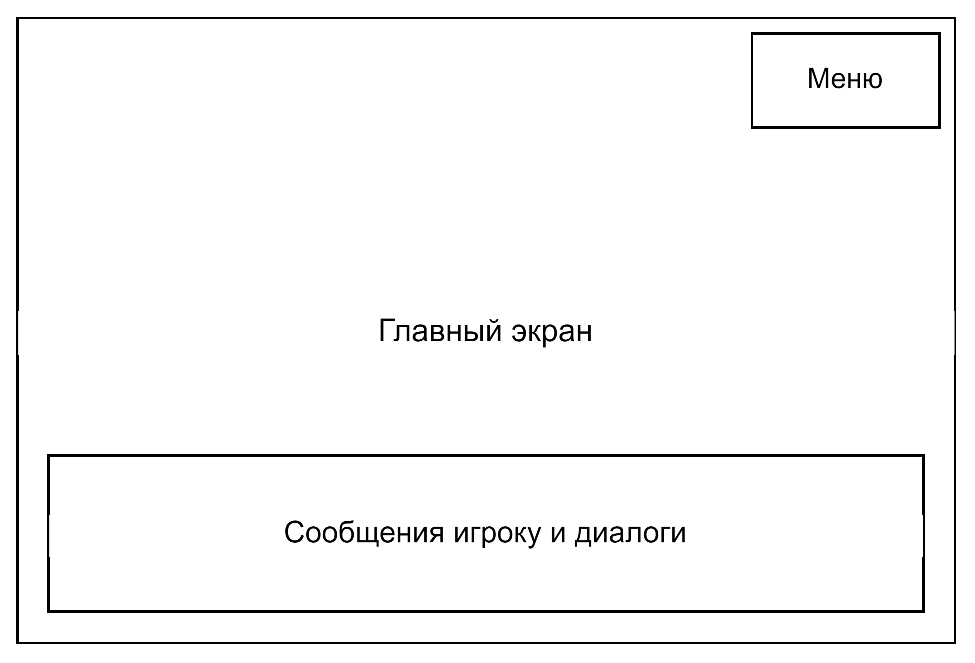
\includegraphics[width=1\linewidth]{maket}
	\caption{Композиция шаблона интерфейса игры}
	\label{maket:image}
\end{figure}
%\vspace{-\figureaboveskip} % двойной отступ не нужен (можно использовать, если раздел заканчивается картинкой)

\subsection{Пример игры}
 \begin{itemize}
 	\item ролевая игра моделирует все основные механики Dungeons and Dragons, в которой игрок управляет персонажем, который бродит по одноуровневому подземелью, собирая сокровища и убивая монстров. Подземелье визуализируется в двухмерном виде сверху с использованием экранной графики персонажей и управляется с помощью команд с мыши. Подземелье имеет фиксированную планировку, но встречи с монстрами и сокровища генерируются заданным образом.
 	\begin{itemize}
 		\item 1. Цель игры: Основная цель игры заключается в исследовании мира, выполнении заданий и квестов, сражении с врагами и развитии своего персонажа. Игра также имеет главный сюжет, который игрок может прогрессировать, следуя определенным событиям и заданиям
 		\item 2. Боевая система:  Бои могут происходить в режиме реального времени. Игрок может управлять группой персонажей и давать им команды в бою. В бою игрок может использовать различные атаки, заклинания и способности своего персонажа для победы над врагами
 		\item 3. Персонажи: Игрок может создать своего уникального персонажа, выбрав класс, расу, навыки и характеристики. Каждый класс имеет свои особенности и специализации, определяющие стиль игры и возможности персонажа. Персонажи могут повышать уровень, получать новые навыки и способности, улучшать характеристики и собирать экипировки
 		\item 4. Исследование мира: Игрок может свободно перемещаться по миру игры, исследуя различные локации и взаимодействуя с окружающими объектами. Во время исследования игрок может встретить неигровых персонажей (NPC), с которыми можно общаться, получать задания и информацию о мире.
 		\item 5. Прогрессия и развитие: Игрок может зарабатывать опыт и повышать уровень своего персонажа. Повышение уровня позволяет персонажу получать новые навыки, улучшать характеристики и получать новые способности. Игрок также может собирать и улучшать экипировку для своего персонажа, чтобы повысить его силу и выживаемость.
 		\item 6. Задания и квесты: Игрок может выполнять различные задания и квесты, предлагаемые неигровыми персонажами. Задания могут включать поиск предметов, убийство определенных врагов, решение головоломок и т.д. За выполнение заданий игрок может получать награды, опыт и продвигаться в сюжете игры.
 	\end{itemize}
 \end{itemize}
 
\subsection{Особенности Dungeons and Dragons}
\begin{itemize}
	\item Dungeons and Dragons (DnD) - это настольная ролевая игра, в которой игроки сотрудничают вместе, чтобы создать историю в фантастическом мире. В DnD один игрок выступает в роли Мастера игры (Мастера подземелий), который рассказывает и контролирует мир, а остальные игроки играют за своих персонажей, которых они создают и развивают.
	\begin{itemize} Основные элементы ролевой системы DnD включают:
		\item 1. Классы и расы: Классы представляют различные роли и специализации персонажей, такие как воин, маг, жрец. Каждый класс имеет свои уникальные способности и навыки.
			\begin{itemize}
				\item Особенности воина: воин специализируется на ближнем бою, может использовать все виды оружия, может носить все доспехи и щиты, не способен накладывать заклинания, его кость здоровья 10-гранный кубик (D10).
				\item Особенности мага: маг специализируется на дальнем бою, может использовать только боевые посохи и короткие мечи, не может носить доспехи , способен накладывать заклинания, наносящие большое количество урона, его кость здоровья 6-гранный кубик (D6).
				\item Особенности жреца: жрец специализируется на ближнем бою, может использовать простое оружия, может носить лёгкие,средние доспехи и щиты, способен накладывать заклинания, исцеляющие его, его кость здоровья 8-гранный кубик (D8).
			\end{itemize}

		\item Расы определяют происхождение персонажа и дают особые характеристики и способности. Примеры рас включают эльфов, дварфов, людей.
			\begin{itemize}
			\item Особенности человека: человек на старте получает +1 ко всем характеристикам, его размер средний.
			\item Особенности эльфа: эльф получает +2 к ловкости и +1 к мудрости, его размер средний, у эльфа есть тёмное зрение в радиусе 30 футов.
			\item Особенности дварфа: дварф получает +2 к силе и +2 к телосложению, его размер маленький, у дварфа есть тёмное зрение в радиусе 30 футов.
			\end{itemize}
		\item 2. Характеристики:
		\begin{itemize}
			\item Характеристики определяют физические и умственные способности персонажа, такие как сила, ловкость, телосложение, интеллект, мудрость, харизма. Они влияют на способности и успех персонажа в различных ситуациях.
			\item Сила - характеристика влияющая на броски атак рукопашным оружием, а так же на проверки навыков: атлетика.
			\item Ловкость - характеристика влияющая на броски атак совершаемых стрелковым оружием, на класс доспеха персонажа, а так же на проверки навыков: акробатика, ловкость рук, скрытность.
			\item Телосложение - характеристика влияющая на колличество здоровья персонажа.
			\item Интеллект - характеристика влияющая на броски атак совершённых заклинаниями волшебника, а так же на проверки навыков: магия, история, природа, расследование, религия.
			\item Мудрость - характеристика влияющая на броски атак  совершённых заклинаниями жреца, а так же на проверки навыков: восприятие, выживание, проницательность, уход за животными, медицина.
			\item Харизма - характеристика влияющая на общение с не игровыми персонажами, а так же на проверки навыков: выступление, убеждение, обман, запугивание.
		\end{itemize}
		\item 3. Навыки:
		\begin{itemize}
			\item Навыки представляют специализации персонажа в определенных областях, таких как взлом замков, обращение с оружием, магия и т.д. Навыки могут быть использованы для выполнения действий и решения задач
		\end{itemize}
		\item 4. Броски костей:
		\begin{itemize}
			\item Игра DnD использует различные виды игровых костей для случайной генерации результатов. Например, для определения успеха атаки или проверки навыка игрок может бросить 20-гранный кубик (D20) и добавить соответствующие модификаторы.
		\end{itemize}
		\item 5. Приключения и задания:
		\begin{itemize}
			\item Мастер игры создает историю, включающую задания и приключения, которые игроки выполняют. Задания могут включать исследование подземелий, сражение с монстрами, решение головоломок и взаимодействие с неигровыми персонажами.
		\end{itemize}
		\item 6: Прогрессия и опыт:
		\begin{itemize}
			\item Персонажи получают опыт за выполнение заданий и сражение с врагами. Зарабатывая опыт, персонажи повышают уровень, получают новые способности и становятся сильнее.
		\end{itemize}
		\item 7. Магия:
		\begin{itemize}
			\item DnD имеет разветвленную систему магии, позволяющую персонажам использовать заклинания различных уровней и школ. Магические заклинания могут влиять на бой, лечение, обнаружение и другие аспекты игры.
		\end{itemize}
	\end{itemize}
\end{itemize}

\subsection{Интерфейс пользователя}
Создаётся рабочее окно tkinter, на нём пользователь видит текущую зону, из зоны current\_area, так же все объекты, находящиеся в ней, и всех персонажей из команды персонажей, текущей игры. Пользователь может взаимодействовать с окном с помощью мыши. Левым кликом мыши по окну вызывает метод mouse\_click у текущей игры. который вызывает проверку находится ли в координатах, в которых был совершён клик, какой-либо персонаж или объект, и если есть, то вызвать метод on\_click. Если персонажа в данных координатах нет, то вызвать у всех персонажей с полем category == "pc" метод search\_position(x,y), который указывает координаты движения, которые должны прийти персонажи. Так же работают все сценарии, конкретной зоны. они работают до тех пор, пока не будет вызвано условие останавливающее, конкретный сценарий.
\subsection{ Моделирование вариантов использования}
На основании анализа предметной области в программе должны быть реализованы следующие прецеденты:
\begin{enumerate}
\item Создание персонажа.
\item Создание зоны.
\item Создание объекта.
\item Удаление объекта.
\item Создание сценария.
\item Удаление сценария.
\end{enumerate}
Таким образом, на рисунке ~\ref{prec:image}сформированы следующие действия пользователя и их последствия.
\begin{figure}[ht]
	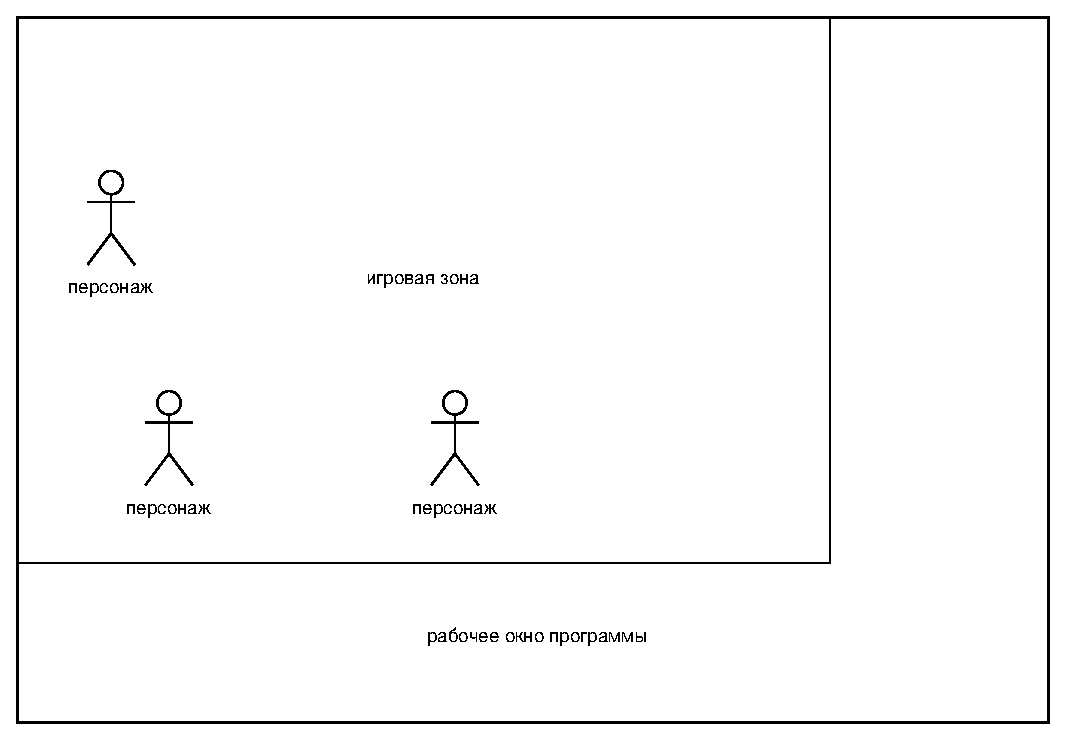
\includegraphics[width=1\linewidth]{prec}
	\caption{Шаблон интерфейса игры}
	\label{prec:image}
\end{figure}
%\vspace{-\figureaboveskip} % двойной отступ не нужен (можно использовать, если раздел заканчивается картинкой)

\subsection{Требования к оформлению документации}

Разработка программной документации и программного изделия должна производиться согласно ГОСТ 19.102-77 и ГОСТ 34.601-90. Единая система программной документации.

\section{Технический проект}
\subsection{Общая характеристика организации решения задачи}

Необходимо спроектировать и разработать приложение, который должен способствовать популяризации ролевых игр.

Приложение представляет собой набор взаимосвязанных различных окон, которые сгруппированы по разделам, содержащие текстовую, графическую информацию. Приложение располагается на компьютере.

\subsection{Обоснование выбора технологии проектирования}

На сегодняшний день информационный рынок, поставляющий программные решения в выбранной сфере, предлагает множество продуктов, позволяющих достигнуть поставленной цели – разработки приложения.

\subsubsection{Описание используемых технологий и языков программирования}

В процессе разработки приложения используются программные средства и языки программирования. Каждое программное средство и каждый язык программирования применяется для круга задач, при решении которых они необходимы.

\subsubsection{Язык программирования Python}

Python –  высокоуровневый язык программирования общего назначения с динамической строгой типизацией и автоматическим управлением памятью, ориентированный на повышение производительности разработчика, читаемости кода и его качества, а также на обеспечение переносимости написанных на нём программ. Язык является полностью объектно-ориентированным в том плане, что всё является объектами. Необычной особенностью языка является выделение блоков кода отступами. Синтаксис ядра языка минималистичен, за счёт чего на практике редко возникает необходимость обращаться к документации. Сам же язык известен как интерпретируемый и используется в том числе для написания скриптов. Недостатками языка являются зачастую более низкая скорость работы и более высокое потребление памяти написанных на нём программ по сравнению с аналогичным кодом, написанным на компилируемых языках, таких как C или C++.

\subsubsection{Использование библиотеки Tkinter и реализация таймеров на Python}
	
\paragraph{Введение}
Библиотека Tkinter - это стандартная библиотека Python для создания графического пользовательского интерфейса (GUI). Она обладает широкими возможностями для создания разнообразных приложений с использованием различных виджетов, таких как кнопки, поля ввода, метки и многое другое.
	
\paragraph{Возможности Tkinter}
Вот некоторые из основных возможностей, предоставляемых библиотекой Tkinter:
	
\begin{itemize}
	\item Создание различных виджетов: кнопки, метки, поля ввода, списки и многое другое.
	\item Управление компоновкой виджетов с использованием менеджеров компоновки (например, grid, pack, place).
	\item Обработка событий, таких как щелчок мыши, нажатие клавиш и другие.
	\item Возможность создания различных диалоговых окон, таких как окна предупреждений, информационные окна и окна запроса.
	\item Поддержка многопоточности для обновления интерфейса из различных потоков выполнения.
\end{itemize}
	
\paragraph{Реализация таймеров на Python}
Для реализации таймеров на Python можно использовать модуль \texttt{time} или \texttt{threading}. Вот пример использования модуля \texttt{time} для создания простого таймера:
	
	import time\\
	
	def countdown(t):\\
	while t > 0:\\
	mins, secs = divmod(t, 60)\\
	timeformat = '{:02d}:{:02d}'.format(mins, secs)\\
	print(timeformat, end='\r')\\
	time.sleep(1)\\
	t -= 1\\
	print('Таймер завершен!')\\
	

	t = 10v
	countdown(t)\\
	
Этот код создает простой обратный отсчет таймера с использованием функции \texttt{countdown}. Он выводит оставшееся время в формате ММ:СС и уменьшает его на 1 каждую секунду, используя функцию \texttt{time.sleep(1)}. Когда время истекает, выводится сообщение о завершении таймера.
	
\paragraph{Заключение}
Библиотека Tkinter предоставляет мощные инструменты для создания графических пользовательских интерфейсов на языке Python. Реализация таймеров на Python может быть достигнута с помощью модулей \texttt{time} или \texttt{threading}, в зависимости от конкретных требований приложения.

\subsection{Описание платформы для создания RPG игр}
Клиент создает модуль содержащий методы модуля RPGGame, например bggame. В этом модуле мы создаем мир игры, с помощью new\_actor. Мы можем вызывать их много раз с разными параметрами, или загрузить параметры для этих функций из файла. После чего у нас есть персонажи и предметы. Мир также состоит из зон (Area). Каждая зона включает в себя графику, персонажи и предметы и сценарии взаимодействия. Исключение составляет команда PC, которая может перемещаться из зоны в зону (это мы программируем у клиента). Команду мы тоже определяем стартовую и впоследствии можем менять (add\_actor\_to\_team, remove\_actor\_from\_team). Каждому персонажу и объекту может соответствовать пользовательский сценарий (он активируется при нажатии мышкой на объект). Сценарий может включать диалог, взятие предмета, добавление персонажа в команду, квест и т.д.
Зона тоже может содержать сценарий, который запускается когда команда попадает в зону.
Клиентский класс (BGGame) также содержит глобальные переменные, определяющие ситуации в игре (например квесты). Локальные переменные могут быть в зоне.

Как программируются зоны. Если нужны локальные переменные (состояние локальных событий), то тогда нужно создавать класс своей зоны как наследник от Area. Или же просто использовать класс Area. Добавляем зону в игру new\_area(name, area). Переключаем зону - set\_area(name). Глобальные сценарии находятся в классе игры (BGGame), мы подключаем их как :
Area.set\_enter\_script(script)
В зону мы добавляем персонажей и предметы как add\_object(x,y, obj) - z не нужно, так как слой можно определить по y координате.
В конкретную зону мы добавляем сценарий для взаимодействия как: Game.game.start\_script(script, name)
Как происходит переход команды между зонами.
В зоне определяем объект дверь, по клику мыши она может открываться и закрываться (меняется состояние объекта). Назначаем сценарий walk\_script(script), который срабатывает когда кто-то из команды пересекает объект. В этом сценарии мы меняем зону на нужную (set\_area), и устанавливаем команду в нужную позицию (set\_team). В другой зоне делается аналогично, только переход и позиция будут другими.
Сценарии - это потоки которые запускаются параллельно (метод RPGGame.start\_script(script)). Сценарий может быть остановлен (stop\_script(name)).
Таким образом, мир будет интерактивным.
Как связано окно и графика с игрой. В окне мы делаем таймер, который вызывает метод update нашей игры (BGGame). Этот метод выполняет все действия объектов в игре за 1 кадр времени.
Также в таймере вызываем Graphics.update(), который обновляет графику игры.
Все объекты (Actor, Item) должны иметь состояния (как минимум одно). Каждое состояние связано с спрайтом (или анимацией). То есть переключение состояния меняет графику объекта.

А вообще сценарии и глобальные переменные могут быть без классов, а просто в модулях, так проще, чтобы к ним был доступ из всех комнат. Тогда и функции движка должны быть доступны везде (то есть во всех сценариях). Например делаем модуль руины (ruins):
import random\\
from math import sqrt\\
import time\\
from rpg.area import *\\
from rpg.sprite import *\\
from rpg.rectangle import *\\
from rpg.game import Game\\
from rpg.portal import Portal\\

class Ruins(Area):\\
def \_\_init\_\_(self):\\
'''\\
Класс игровой зоны Ruins\\

'''\\
super().\_\_init\_\_()\\
self.add\_sprite(Sprite('images/fon3.png'), 590, 400, 0)\\
self.add\_rect(Rectangle(x=0, y=0, width=Sprite('images/fon3.png').image.width(), height=Sprite('images/fon3.png').image.height()))\\
from grunt import Grunt\\
self.grunt = Grunt(0,0,0)\\
from footman import Footman\\
self.footman = Footman(0,0,0)\\
self.add\_object(self.footman, 120, 120, 1)\\
self.add\_object(self.grunt, 500, 185, 1)\\
p = Portal(400, 400, 200, 200, 'Village', 480, 100)\\
self.add\_object(p, p.pos\_x, p.pos\_y, 100)\\
Game.game.start\_script(self.ai, "ai", self.grunt)\\
Game.game.start\_script(self.walk\_two, "footman", 50, 50)\\


def walk(self, step\_x, step\_y, actor):\\
'''\\
Сценарий для движения бугая\\

:param step\_x: шаг движения x\\
:param step\_y: шаг движения y\\
'''\\
if actor.hp <= 0:\\
Game.game.stop\_script("grunt")\\
new\_x = 200\\
new\_y = 200\\
actor.is\_attack = False\\
direction = random.choice(["up", "down", "left", "right"])\\
if direction == "up":\\
new\_y -= step\_y\\
new\_x = step\_x\\
elif direction == "down":\\
new\_y += step\_y\\
new\_x = step\_x\\
elif direction == "left":\\
new\_y = step\_y\\
new\_x -= step\_x\\
elif direction == "right":\\
new\_y = step\_y\\
new\_x += step\_x\\

actor.search\_position(new\_x, new\_y)\\

time.sleep(2)\\

модуль bggame:\\
from ruins import *\\
import time\\
import random\\

class BaldursGame(Game):\\
def \_\_init\_\_(self, canvas, window, **params):\\
'''\\
Класс конкретной игры для демонстрации\\

:param canvas: класс графической системы\\
:param window: окно на которое будет выводится игра\\
'''\\
super().\_\_init\_\_(canvas, window, **params)\\
from mage import Mage\\
self.add\_pc\_to\_team(Mage(0, 0, 0))\\
self.new\_area('Ruins', Ruins())\\
self.set\_area('Ruins')\\
self.set\_team(500, 300, 100)\\
self.timer()\\

\subsubsection{Пример клиентского кода игры}
\paragraph{Cоздание классов персонажей/предметов}
Клиент создает модуль содержащий методы модуля RPGGame, например BaldursGateGame. В этом модуле клиент создаем мир игры, с помощью new\_actor. 

модуль bggame:\\
from ruins import *\\
import time\\
import random\\

class BaldursGame(Game):\\
def \_\_init\_\_(self, canvas, window, **params):\\
'''\\
Класс конкретной игры для демонстрации\\

:param canvas: класс графической системы\\
:param window: окно на которое будет выводится игра\\
'''\\
super().\_\_init\_\_(canvas, window, **params)\\
from mage import Mage\\
self.add\_pc\_to\_team(Mage(0, 0, 0))\\
self.new\_area('Ruins', Ruins())\\
self.set\_area('Ruins')\\
self.set\_team(500, 300, 100)\\
self.timer()\\

\paragraph{Задание правил атаки}
Пользователь создаёт класс ADnDActor, наследник от класса Actor в своём модуле bggame, в нём он прописывает свои правила по которым происходит атака. То есть Actor.attack(self, actor), где actor - кого атакуют.
Пример:

модуль adnd\_actor:\\
from math import sqrt\\
from rpg.actor import Actor\\
from rpg.animation import Animation\\
import rpg.game\\
import time\\

class Adnd\_actor(Actor):\\

ATTACK\_RANGE = 50\\

def \_\_init\_\_(self, x, y, z, **params):\\
'''\\
Класс Adnd\_actor содержащий основные механики взаимодействия с другими персонажами\\

:param x: координата x\\
:param y: координата y\\
:param z: координата z\\
'''\\
super().\_\_init\_\_(x, y, z, **params)\\
self.on\_click = self.click\\

def click(self):\\
'''\\
вызывается при клике на персонажа\\

'''\\
pc = rpg.game.Game.game.team\_of\_pc[0]\\
if pc == self:\\
return\\
dx = pc.pos\_x - self.pos\_x\\
dy = pc.pos\_y - self.pos\_y\\
dist = sqrt(dx * dx + dy * dy)\\
if dist <= self.ATTACK\_RANGE:\\
pc.is\_attack = True\\
pc.attack(self)\\
time.sleep(0.125)\\
if self.hp <=0:\\
pc.is\_attack = False\\

def attack(self, actor):\\
'''\\
совершает атаку по actor\\

:param actor: персонаж, которого атакуют\\
'''\\
actor.hp -= self.damage\\
def update(self):\\
'''\\
обновляет состояние персонажа\\

'''\\
super().update()\\
if self.hp <= 0:\\
self.stop\_move()\\
self.set\_state('death')\\


\paragraph{Создание зон, заполнение их персонажами/объектами}
Мир также состоит из зон (Area). Каждая зона включает в себя графику, персонажи и предметы и сценарии взаимодействия. Исключение составляет команда PC, которая может перемещаться из зоны в зону (это мы программируем у клиента). Как программируются зоны. Если нужны локальные переменные (состояние локальных событий), то тогда нужно создавать класс своей зоны как наследник от Area. Или же просто использовать класс Area. Добавляем зону в игру new\_area(name, area). Переключаем зону - set\_area(name). Так же требуется задать область движения, её проще сделать как совокупность прямоугольников, за которые персонажи не могут выйти. Эти прямоугольники должны касаться друг друга, но не пересекаться. Тогда алгоритм проверки выхода несложный: выход за пределы области только тогда, когда прямоугольник персонажа пересек сторону (одну или две) одного из прямоугольников области, эта сторона не является касательной.

import random\\
from math import sqrt\\
import time\\
from rpg.area import *\\
from rpg.sprite import *\\
from rpg.rectangle import *\\
from rpg.game import Game\\
from rpg.portal import Portal\\

class Ruins(Area):\\
def \_\_init\_\_(self):\\
'''\\
Класс игровой зоны Ruins\\

'''\\
super().\_\_init\_\_()\\
self.add\_sprite(Sprite('images/fon3.png'), 590, 400, 0)\\
self.add\_rect(Rectangle(x=0, y=0, width=Sprite('images/fon3.png').image.width(),\\ height=Sprite('images/fon3.png').image.height()))
from grunt import Grunt\\
self.grunt = Grunt(0,0,0)\\
from footman import Footman\\
self.footman = Footman(0,0,0)\\
self.add\_object(self.footman, 120, 120, 1)\\
self.add\_object(self.grunt, 500, 185, 1)\\
p = Portal(400, 400, 200, 200, 'Village', 480, 100)\\
self.add\_object(p, p.pos\_x, p.pos\_y, 100)\\
Game.game.start\_script(self.ai, "ai", self.grunt)\\
Game.game.start\_script(self.walk\_two, "footman", 50, 50)\\


def walk(self, step\_x, step\_y, actor):\\
'''\\
Сценарий для движения бугая\\

:param step\_x: шаг движения x\\
:param step\_y: шаг движения y\\
'''\\
if actor.hp <= 0:\\
Game.game.stop\_script("grunt")\\
new\_x = 200\\
new\_y = 200\\
actor.is\_attack = False\\
direction = random.choice(["up", "down", "left", "right"])\\
if direction == "up":\\
new\_y -= step\_y\\
new\_x = step\_x\\
elif direction == "down":\\
new\_y += step\_y\\
new\_x = step\_x\\
elif direction == "left":\\
new\_y = step\_y\\
new\_x -= step\_x\\
elif direction == "right":\\
new\_y = step\_y\\
new\_x += step\_x\\

actor.search\_position(new\_x, new\_y)\\

time.sleep(2)\\

модуль bggame:\\
from ruins import *\\
import time\\
import random\\

\paragraph{Пример сценариев: переход между зонами}
Глобальные сценарии находятся в классе игры (BGGame), мы подключаем их как :
Area.set\_enter\_script(script)\\
Как происходит переход команды между зонами.
В зоне определяем объект портал, по клику мыши когда персонаж заходит внутрь портала срабатывает self.actor\_in(self, actor). При создании портала, мы указываем кудаи в какую зону разместить команду персонажей.

from rpg.object import Object\\
from rpg.game import Game\\
from rpg.rectangle import Rectangle\\

class Portal(Object):\\
def \_\_init\_\_(self, x, y, width, height, area, team\_x, team\_y):\\
''' \\
Создает портал в новую зону\\

:param x: координата x портала\\
:param y: координата y портала\\
:param width: ширина портала\\
:param height: высота портала\\
:param area: имя зоны куда будет переход\\
:param team\_x: местоположение команды в новой зоне\\
:param team\_y: местоположение команды в новой зоне\\
'''\\
self.states = None\\
self.sprite = None\\
self.category = 'portal'\\
super().\_\_init\_\_(x, y, 0)\\
self.rectangle = Rectangle(x, y, width, height)\\
self.area = area\\
self.team\_x = team\_x\\
self.team\_y = team\_y\\
self.visible = False\\

def actor\_in(self, actor):\\
'''\\
Проверяет находится ли персонаж внутри портала\\

:param actor: проверяемый персонаж\\
'''\\
if actor.category == "pc":\\
Game.game.set\_area(self.area)\\
Game.game.set\_team(self.team\_x, self.team\_y, 100)\\
actor.stop\_move()\\

модуль ruins\\
import random\\
from math import sqrt\\
import time\\
from rpg.area import *\\
from rpg.sprite import *\\
from rpg.rectangle import *\\
from rpg.game import Game\\
from rpg.portal import Portal\\

class Ruins(Area):\\
def \_\_init\_\_(self):\\
'''\\
Класс игровой зоны Ruins\\

'''\\
super().\_\_init\_\_()\\
self.add\_sprite(Sprite('images/fon3.png'), 590, 400, 0)\\
self.add\_rect(Rectangle(x=0, y=0, width=Sprite('images/fon3.png').image.width(), height=Sprite('images/fon3.png').image.height()))\\
from grunt import Grunt\\
self.grunt = Grunt(0,0,0)\\
from footman import Footman\\
self.footman = Footman(0,0,0)\\
self.add\_object(self.footman, 120, 120, 1)\\
self.add\_object(self.grunt, 500, 185, 1)\\
p = Portal(400, 400, 200, 200, 'Village', 480, 100)\\

\paragraph{Как будет идти бой}
Бой будет совершаться с помощью сценариев. У класса Adnd\_actor есть метод attack(self, actor), который уменьшает текущее количество здоровья у actor. В модуле game существуют методы start\_script(script, name), stop\_script(name). С помощь сценариев возможно запускать параллельные потоки. В конкретную зону будет добавляться сценарий 'ai', в который передаётся конкретный персонаж. В этом сценарии указывается поведение противника, Что он должен сближаться с персонажем игрока, и когда расстояние до атаки будет достаточным, чтобы её совершить, будет вызван метод actor.attack. Для того, чтобы пользователь мог атаковать персонажа, у каждого экземпляра класса adnd\_actor есть метод click(self), который вызывает проверку условия, если персонаж близко к персонажу игрока, хранящемуся в rpg.game.Game.team\_of\_pc, то вызвать у pc=rpg.game.Game.team\_of\_pc[0], attack(self)/
Пример:
модуль adnd\_actor:\\
from math import sqrt\\
from rpg.actor import Actor\\
from rpg.animation import Animation\\
import rpg.game\\
import time\\

class Adnd\_actor(Actor):\\

ATTACK\_RANGE = 50\\

def \_\_init\_\_(self, x, y, z, **params):\\
'''\\
Класс Adnd\_actor содержащий основные механики взаимодействия с другими персонажами\\

:param x: координата x\\
:param y: координата y\\
:param z: координата z\\
'''\\
super().\_\_init\_\_(x, y, z, **params)\\
self.on\_click = self.click\\

def click(self):\\
'''\\
вызывается при клике на персонажа\\

'''\\
pc = rpg.game.Game.game.team\_of\_pc[0]\\
if pc == self:\\
return\\
dx = pc.pos\_x - self.pos\_x\\
dy = pc.pos\_y - self.pos\_y\\
dist = sqrt(dx * dx + dy * dy)\\
if dist <= self.ATTACK\_RANGE:\\
pc.is\_attack = True\\
pc.attack(self)\\
time.sleep(0.125)\\
if self.hp <=0:\\
pc.is\_attack = False\\

def attack(self, actor):\\
'''\\
совершает атаку по actor\\

:param actor: персонаж, которого атакуют\\
'''\\
actor.hp -= self.damage\\
def update(self):\\
'''\\
обновляет состояние персонажа\\

'''\\
super().update()\\
if self.hp <= 0:\\
self.stop\_move()\\
self.set\_state('death')\\

модуль ruins\\
import random\\
from math import sqrt\\
import time\\
from rpg.area import *\\
from rpg.sprite import *\\
from rpg.rectangle import *\\
from rpg.game import Game\\
from rpg.portal import Portal\\

class Ruins(Area):\\
def \_\_init\_\_(self):\\
'''\\
Класс игровой зоны Ruins\\

'''\\
super().\_\_init\_\_()\\
self.add\_sprite(Sprite('images/fon3.png'), 590, 400, 0)\\
self.add\_rect(Rectangle(x=0, y=0, width=Sprite('images/fon3.png').image.width(), height=Sprite('images/fon3.png').image.height()))\\
from grunt import Grunt\\
self.grunt = Grunt(0,0,0)\\
from footman import Footman\\
self.footman = Footman(0,0,0)\\
self.add\_object(self.footman, 120, 120, 1)\\
self.add\_object(self.grunt, 500, 185, 1)\\
p = Portal(400, 400, 200, 200, 'Village', 480, 100)\\
self.add\_object(p, p.pos\_x, p.pos\_y, 100)\\
Game.game.start\_script(self.ai, "ai", self.grunt)\\
Game.game.start\_script(self.walk\_two, "footman", 50, 50)\\


def walk(self, step\_x, step\_y, actor):\\
'''\\
Сценарий для движения бугая\\

:param step\_x: шаг движения x\\
:param step\_y: шаг движения y\\
'''\\
if actor.hp <= 0:\\
Game.game.stop\_script("grunt")\\
new\_x = 200\\
new\_y = 200\\
actor.is\_attack = False\\
direction = random.choice(["up", "down", "left", "right"])\\
if direction == "up":\\
new\_y -= step\_y\\
new\_x = step\_x\\
elif direction == "down":\\
new\_y += step\_y\\
new\_x = step\_x\\
elif direction == "left":\\
new\_y = step\_y\\
new\_x -= step\_x\\
elif direction == "right":\\
new\_y = step\_y\\
new\_x += step\_x\\

actor.search\_position(new\_x, new\_y)\\

def ai(self, actor):\\
'''\\
скрипт противников\\

:param step\_x: размер шага x до персонажа игрока\\
:param step\_y: размер шага x до персонажа игрока\\
:param actor: персонаж противник\\
'''\\
if actor.hp <= 0:\\
Game.game.stop\_script("ai")\\
import rpg.game\\
pc = rpg.game.Game.game.team\_of\_pc[0]\\
new\_x = pc.pos\_x\\
new\_y = pc.pos\_y\\

actor.search\_position(new\_x, new\_y)\\
dx = pc.pos\_x - actor.pos\_x\\
dy = pc.pos\_y - actor.pos\_y\\
dist = sqrt(dx * dx + dy * dy)\\
if dist <= actor.ATTACK\_RANGE:\\
actor.is\_attack = True\\
actor.attack(pc)\\
time.sleep(1)\\
if pc.hp <=0:\\
actor.update()\\
Game.game.stop\_script("ai")\\
Game.game.start\_script(self.walk, "grunt", 50, 50, actor)\\

else:\\
actor.is\_attack = False\\
time.sleep(2)\\

\paragraph{Соединение движка и окон tkinter}
Модуль graphics содержит в себе библиотеку tkinter . Класс Graphics внутри модуля является наследником tk.Canvas. Этот класс взаимодействует с окном root = tk.TK() в программном модуле пользователя. Модуль sprite тоже взаимодействует с tkinter. Изображение для спрайта берётся с помощью метода tk.PhotoImage(file=name)

модуль sprite\\

import tkinter as tk\\
class Sprite:\\

def \_\_init\_\_(self, image):\\
'''\\
Класс спрайта для работы с изображениями на Canvas\\

:param image: адресс изображения который\\
'''\\
self.image = tk.PhotoImage(file=image)\\
self.tag = None\\
self.x = 0\\
self.y = 0\\
self.z = 0\\

def set\_tag(self, tag):\\
'''\\
Устанавливает тег спрайта\\

:param tag: тег спрайта\\
'''\\
self.tag = tag\\

def set\_z(self, z):\\
'''\\
Устанавливает z-координату спрайта\\

:param z: координата z\\
'''\\
self.z = z\\

def get\_tag(self):\\
'''\\
Возвращает тег спрайта\\

'''\\
return self.tag\\

def set\_coords(self, new\_x, new\_y):\\
'''\\
Обновляет координаты спрайта\\

:param new\_x: координата x\\
:param new\_y: координата y\\
'''\\
if self.tag:\\
self.x = new\_x\\
self.y = new\_y\\
def update(self):\\
'''\\
Обновляет анимацию спрайта\\

'''\\
pass\\

модуль graphics\\

import tkinter as tk\\

class Graphics(tk.Canvas):\\
canvas = None\\
def \_\_init\_\_(self, master, **kwargs):\\
'''\\
Класс с методами для работы со спрайтами\\

'''\\
super().\_\_init\_\_(master, **kwargs)\\
self.sprites = []\\
Graphics.canvas = self\\

def add\_sprite(self, sprite, x, y, z, **kwargs):\\
'''\\
Добавляет спрайт на Canvas\\

:param sprite: спрайт
:param x: координата x\\
:param y: координата y\\
:param z: координата z\\
:param kwargs: параметры относящиеся к конкретному изображению в tkinter\\
'''\\
tag = self.create\_image(x, y, image=sprite.image, anchor='center', **kwargs)\\
sprite.set\_tag(tag)\\
sprite.set\_z(z)\\
sprite.x = x\\
sprite.y = y\\
self.sprites.append(sprite)\\
self.sprites.sort(key=lambda sprite: sprite.z)\\

def update(self):\\
'''\\
Перерисовывает все спрайты\\

'''\\
for sprite in self.sprites:\\
sprite.update()\\
self.tag\_raise(sprite.get\_tag())\\
self.coords(sprite.get\_tag(), sprite.x, sprite.y)\\
self.itemconfig(sprite.get\_tag(), image=sprite.image)\\


def change\_sprite(self, sprite, new\_sprite):\\
'''
Меняет  спрайт на новый.\\

:param sprite: экземпляр спрайта\\
:param new\_sprite: новый спрайт\\
'''
old\_sprite\_pos = None\\
for i, s in enumerate(self.sprites):\\
if s.get\_tag() == sprite.get\_tag():\\
old\_sprite\_pos = i\\
break\\

if old\_sprite\_pos is not None:\\
old\_tag = sprite.get\_tag()\\

self.sprites[old\_sprite\_pos] = new\_sprite\\
new\_sprite.set\_tag(old\_tag)\\

new\_sprite.set\_tag(old\_tag)\\
new\_sprite.set\_z(sprite.z)\\

self.tag\_raise(old\_tag)
self.coords(old\_tag, sprite.x, sprite.y)\\
self.itemconfig(old\_tag, image=new\_sprite.image)\\

def delete\_sprite(self, sprite):\\
'''
Удаляет спрайт с Canvas.\\

:param sprite: экземпляр спрайта\\
:return:\\
'''\\
self.delete(sprite.get\_tag())\\
self.sprites.remove(sprite)\\

def clear\_all(self):\\
'''\\
Удаляет все спрайты с Canvas\\

'''\\
for sprite in self.sprites:\\
self.delete(sprite.get\_tag())\\
self.sprites.clear()\\

модуль baldursgame '''пользовательский модуль'''\\

from ruins import *\\
from village import *\\
import time\\
import random\\

class BaldursGame(Game):\\
def \_\_init\_\_(self, canvas, window, **params):\\
'''\\
Класс конкретной игры для демонстрации\\

:param canvas: класс графической системы\\
:param window: окно на которое будет выводится игра\\
'''\\
super().\_\_init\_\_(canvas, window, **params)\\
from mage import Mage\\
self.add\_pc\_to\_team(Mage(0, 0, 0))\\
self.new\_area('Ruins', Ruins())\\
self.new\_area('Village', Village())\\
self.set\_area('Ruins')\\
self.set\_team(500, 300, 100)\\
self.timer()\\

модуль main\\
from bggame import *\\

root = tk.Tk()\\
root.geometry('1500x1500')\\

exit\_button = tk.Button(root, text="Exit", fg="red", command=root.destroy)\\
canvas = Graphics(root, width=1500, height=1500)\\
Graphics.canvas = canvas\\

BaldursGame(canvas, root)\\

canvas.place(height = 1500, width =1500)\\
BaldursGame.timer\\

root.mainloop()

\subsection{Архитектура платформы для создания ролевых игр}
\subsubsection{Диаграмма компонентов классов}
Диаграмма компонентов описывает особенности физического представления разрабатываемой системы. Она позволяет определить архитектуру системы, установив зависимости между программными компонентами, в роли которых может выступать как исходный, так и исполняемый код. Основными графическими элементами диаграммы компонентов являются компоненты, интерфейсы, а также зависимости между ними. На рисунке \ref{diagram.eps:image} изображена диаграмма компонентов для проектируемой системы. Она включает в себя основной класс платформы игры Game и производные от него классы, класс Object с наследниками и их параметрами (полями и методами).
\begin{figure}[ht]
	\center{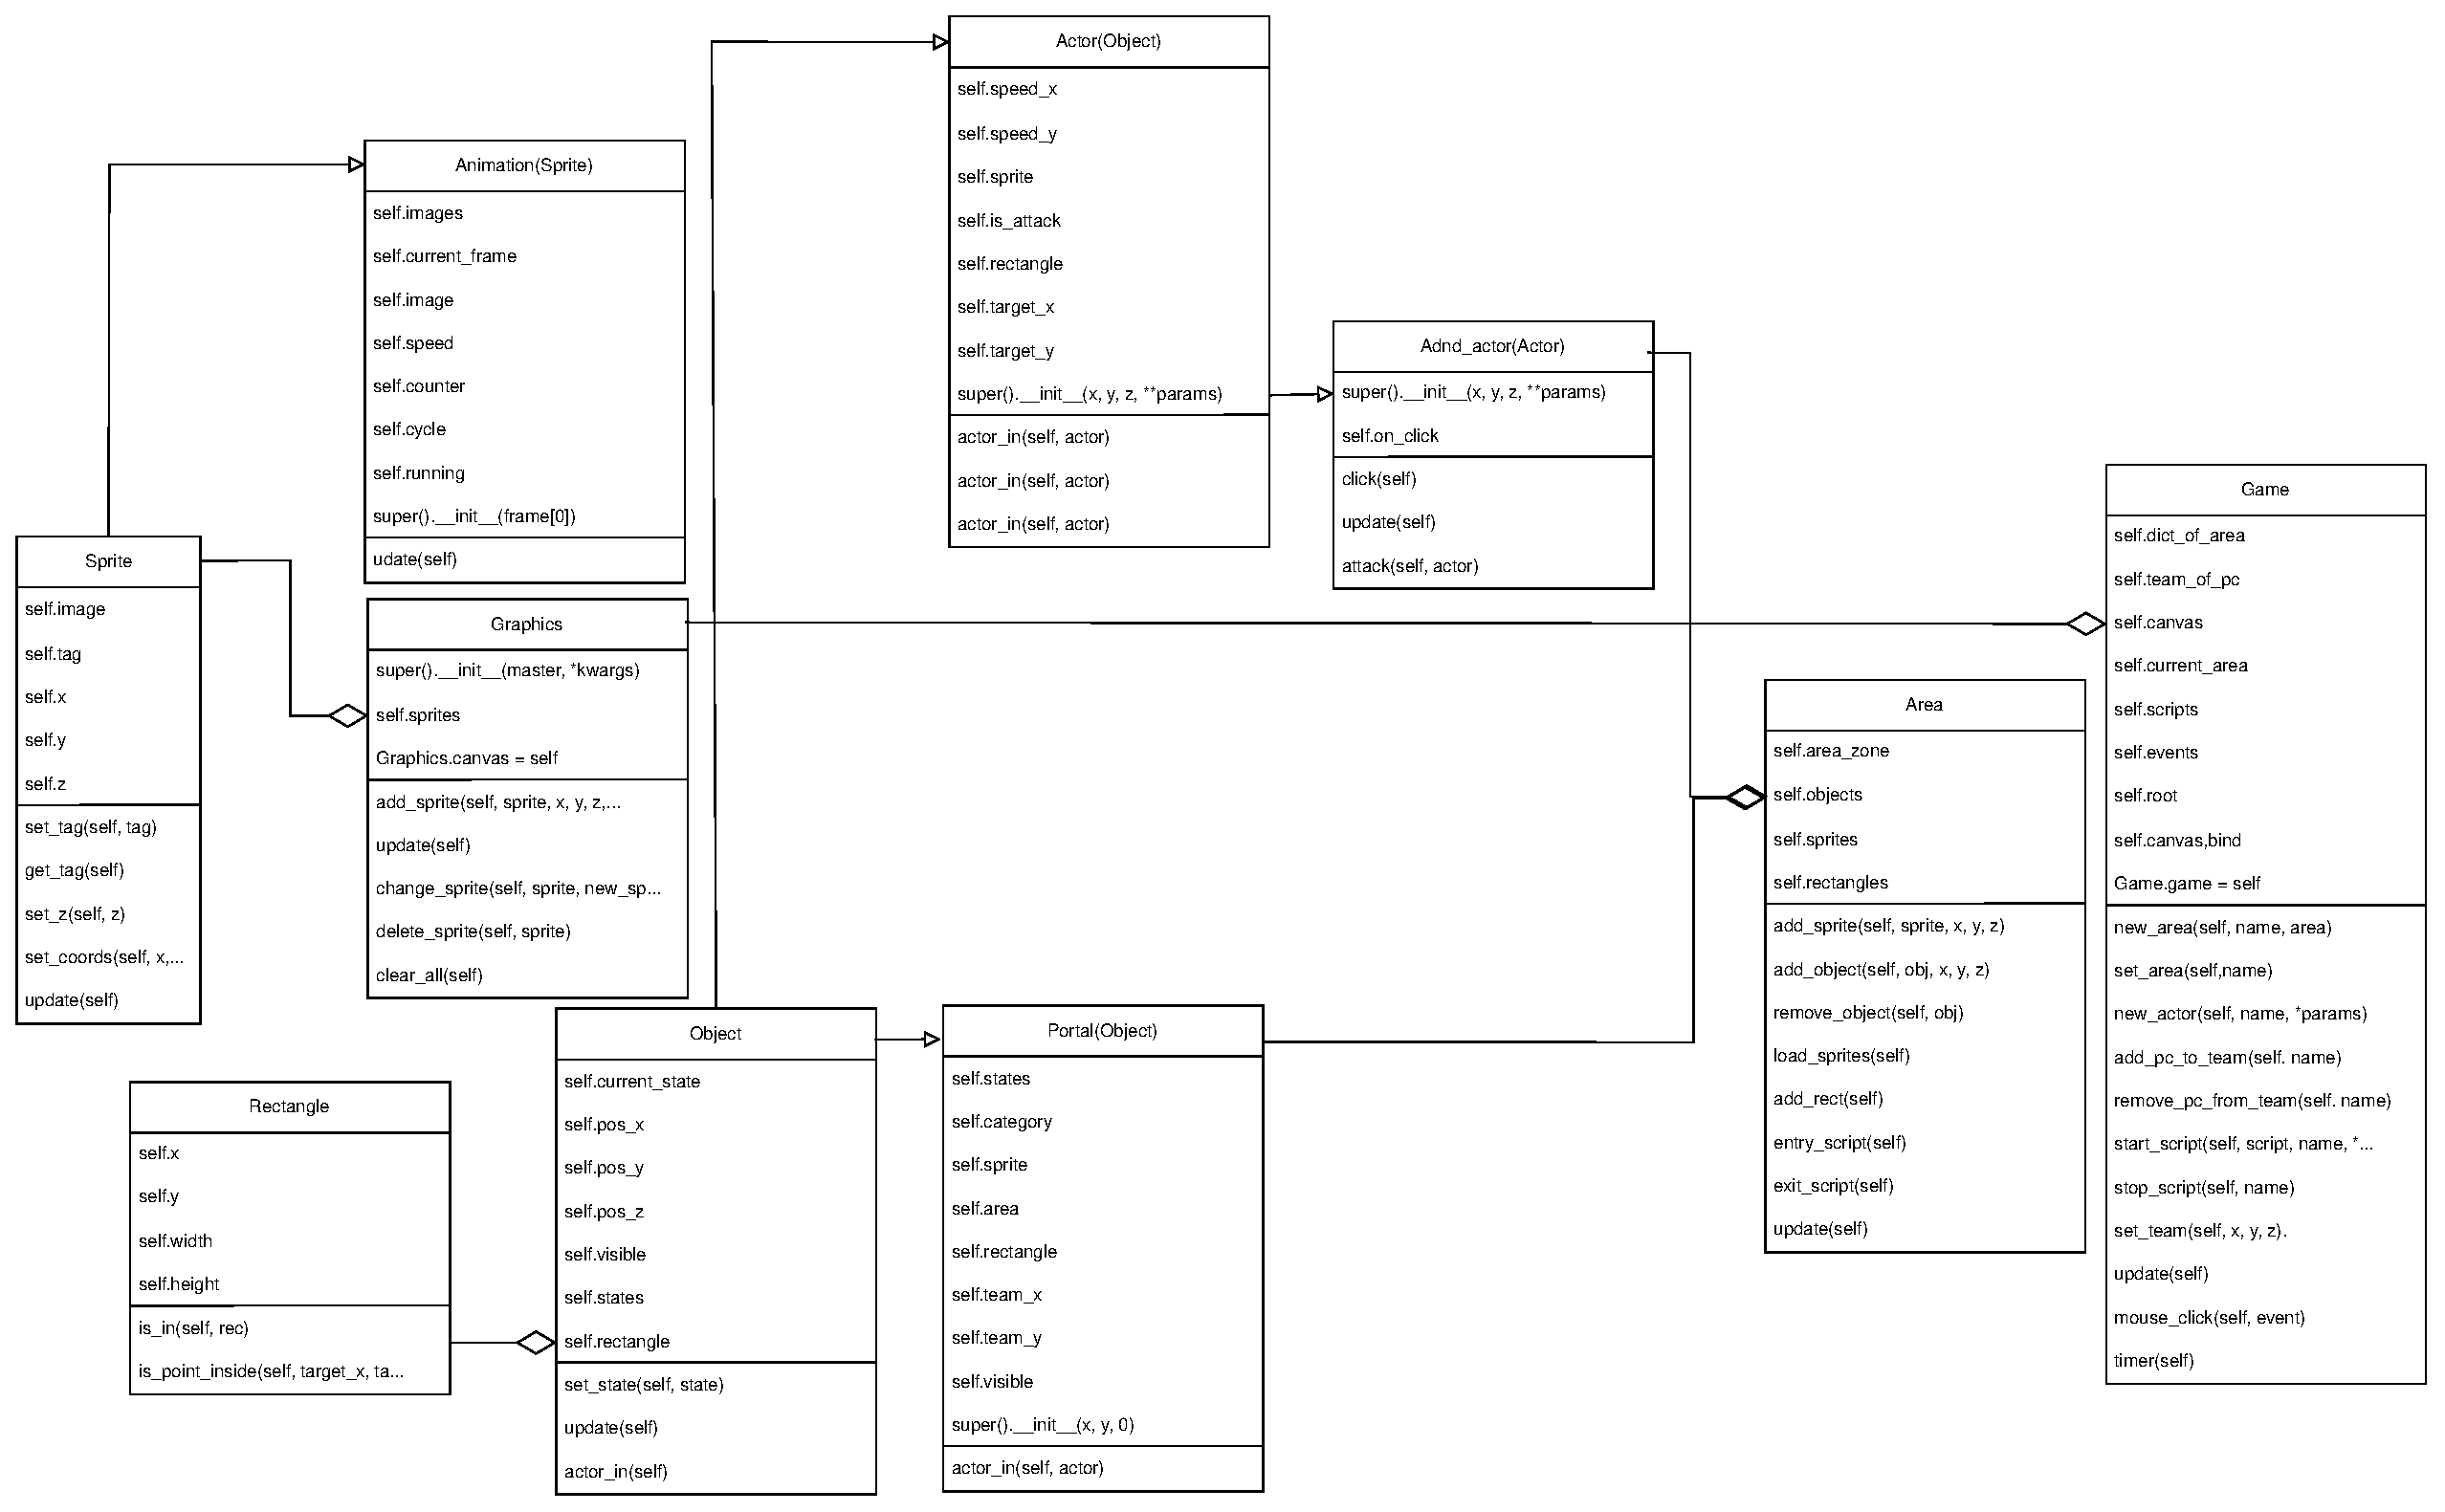
\includegraphics[width=1\linewidth]{diagram}}
	\caption{Диаграмма компонентов}
	\label{diagram:image}
\end{figure}
\paragraph{Описание классов}
\begin{enumerate}
	\item[Graphics] - класс, управляющий спрайтами. Содержит в себе:
	\begin{itemize}
		\item self.sprites - список спрайтов;
		\item add\_sprite(self, sprite x, y, z, image) - добавляет в список спрайт, сохраняет координаты;
		\item change\_sprite(self, sprite new\_sprite) - меняет местами спрайты в списке.
		\item delete\_sprite(self, sprite) - удаляет спрайт из списка.
		\item clear\_all(self) - очищает список спрайтов.
		\item update(self) - добавляет все спрайты из списка на форму.
	\end{itemize}
	\item[Sprite] - класс, хранящий в себе изображение игровых объектов image.
	\begin{itemize}
		\item self.x - координата x.
		\item self.y - координата y.
		\item self.z - координата z.
		\item self.tag - уникальный номер спрайта.
		\item self.image - изображение.
		\item set\_tag(self, tag) - устанавливает tag спрайту.
		\item get\_tag(self) - возвращает tag спрайта.
		\item set\_z(self, z) - устанавливает z координату.
		\item set\_coords(self, new\_x, new\_y) - устанавливает новые координаты.
		\item update(self) - ничего не делает.
	\end{itemize}
	\item[Animation] - класс, хранящий в себе список изображений игровых объектов image. Потомок класса Sprite.
	\begin{itemize}
		\item self.current\_frame - текущий кадр.
		\item self.images  - Загрузка всех кадров анимации.
		\item self.image - Установка начального изображения.
		\item self.speed - скорость анимации.
		\item self.counter - счётчик кадров.
		\item self.cycle - проверка на то что должна ли быть анимация циклично или нет.
		\item self.running - проверка проигрывается ли сейчас анимация.
		\item update(self) - обновляет кадр в анимации.
	\end{itemize}
	\item[Rectangle] - абстрактный класс прямоугольника.
	\begin{itemize}
		\item self.pos\_x - координата x.
		\item self.pos\_y - координата y.
		\item self.width - ширина.
		\item self.height - высота.
		\item is\_in(self, rect) - функция проверки нахождения одного прямоугольника в другом.
		\item is\_point\_inside(self, target\_x, target\_y) - функция проверки точки в пределах прямоугольника.
	\end{itemize}
	\item[Object] - класс, от которого наследуются классы Adnd\_Actor, Actor, Portal.
	\begin{itemize}
		\item self.pos\_x - координата x.
		\item self.pos\_y - координата y.
		\item self.pos\_z - координата z.
		\item self.current\_state - текущее состояние.
		\item self.visible - видимость портала.
		\item self.on\_click - функция клика по объекту.
		\item self.rectangle - прямоугольник объекта.
		\item set\_state(self, state\_name) -устанавливает состояние.
		\item actor\_in(self, actor) - ничего не делает.
		\item update(self) - ничего не делает.
	\end{itemize}
	\item[Portal] - класс объекта для перехода между зонами. Потомок класса Object.
	\begin{itemize}
		\item self.states - состояние портала.
		\item self.sprite - спрайт портала.
		\item self.category - категория.
		\item self.rectangle = - прямоугольник портала.
		\item self.area - зона в которую ведёт портал.
		\item self.team\_x - координата x в  которую нужно разместить команду.
		\item self.team\_y - координата y в  которую нужно разместить команду.
		\item self.visible - видимость портала.
		\item actor\_in(actor) - события, которые произойдут, когда персонаж окажется внутри прямоугольника портала.
	\end{itemize}
	\item[Actor] - класс персонажа, содержащий внутри себя основные поля и методы для перемещения по рабочему окну.
	\begin{itemize}
		\item self.sprite - спрайт персонажа.
		\item self.speed\_x - значение скорости x.
		\item self.speed\_y - значение скорости y.
		\item self.target\_x - координата x в которую должен прийти персонаж.
		\item self.target\_y - координата y в которую должен прийти персонаж.
		\item self.rectangle - прямоугольник персонажа.
		\item self.is\_attack - атакует ли сейчас персонаж.
		\item update(self) - функция обновления координат и состояния персонажа.
		\item search\_position(self, new\_x, new\_y) - поиск координат в которые нужно двигаться персонажу.
		\item stop\_move(self) - остановка движения персонажа.
	\end{itemize}
	\item[Adnd\_Actor] - класс персонажа, содержащий методы связанные с взаимодействием с другими персонажами. Является наследником Actor.
	\begin{itemize}
		\item self.on\_click событие при клике на персонажа
		\item update(self) - функция обновления координат и состояния персонажа.
		\item click(self) - функция вызывается при клике по персонажу.
		\item attack(self, actor) -  функция атаки персонажа по другому персонажу.
	\end{itemize}
	\item[Area] - зона, в которой находятся персонажи и объекты. Содержит следующие поля и методы:
	\begin{itemize}
		\item self.area\_zone - параметр определяющий особенности конкретной зоны.
		\item self.objects - список, хранящий в себе множество объектов.
		\item self.sprites - список фоновых спрайтов.
		\item self.rectangles - прямоугольник зоны.
		\item add\_sprite(self, sprite, x, y, z) - функция добавляет спрайт в зону.
		\item add\_object(self, obj, x, y, z) - функция добавляет объект в зону.
		\item remove\_object(self, obj) - функция удаляет объект из зоны.
		\item load\_sprites(self) - функция загружает все спрайты зоны.
		\item add\_rect(self, rec) - функция добавляет прямоугольник в зону.
		\item entry\_script(self) - функция запускается, когда команда входит в зону.
		\item exit\_script(self) - функция запускается, когда команда выходит из зоны.
		\item update(self) - функция изменяет и проверяет изменение всех объектов в зоне.
	\end{itemize}
	\item[Game] - абстрактный класс, управляющий игрой. Имеет следующие поля и методы:
	\begin{itemize}
		\item self.rpg\_dict\_of\_area - словарь, хранящий в себе множество экземпляров класса Area.
		\item self.team\_of\_pc - список, хранящий в себе имена экземпляров класса Actor с параметром category = "pc".
		\item self.canvas - графика.
		\item self.root - окно для графики.
		\item self.current\_area - параметр хранящий, текущую зону.
		\item self.scripts - словарь для хранения запущенных сценариев.
		\item self.events - словарь для хранения запущенных event`ов сценариев.
		\item self.canvas.bind("<Button-1>", self.mouse\_left.\_click) - обработка клика мыши по рабочему окну.
		\item new\_area(self, name, area) - функция добавляет новую зону в список.
		\item set\_area(self, name) - функция устанавливает текущую зону, загружает графику зоны.
		\item new\_actor(self, name, **params) - функция создаёт класс, потомок от Actor и создаёт поле из параметров, и установление их в начальные значения.
		\item add\_pc\_to\_team(self, pc) - функция добавляет персонажа в команду.
		\item remove\_pc\_from\_team(self, pc) - функция удаляет персонажа из команды.
		\item start\_script(self, script\_function, script\_name, *args) - функция запускает сценарий в отдельном потоке с возможностью остановки и передачи аргументов.
		\item stop\_script(self, script\_name) - функция останавливает сценарий по имени.
		\item set\_team(self, x, y, z) - функция устанавливает координаты персонажей команды.
		\item update(self) - функция вызывается в таймере для обновления всех переменных в текущей зоне.
		\item mouse\_left\_click(self, event) - функция обрабатывает клик мыши.
		\item timer(self) - функция должна вызывать метод update постоянно.
	\end{itemize}
\end{enumerate}

\subsubsection{Реализация графической подсистемы}
Графическая подсистема основана на библиотеке tkinter, которая используется для создания графического интерфейса пользователя. В контексте платформы, tkinter используется для отображения и управления спрайтами — графическими объектами, которые представляют персонажей, предметы и другие элементы игры.
\paragraph{Система спрайтов}
Она реализована через класс Graphics, который расширяет tk.Canvas. Этот класс управляет отображением спрайтов на холсте, их сортировкой по z-координате (что позволяет создать эффект глубины), а также обновлением их позиций. Спрайты могут быть добавлены, перемещены и удалены с холста. Вот пример метода, который добавляет спрайт на холст:

def add\_sprite(self, sprite, x, y, z, **kwargs):\\
tag = self.create\_image(x, y, image=sprite.image, anchor='center', **kwargs)\\
sprite.set\_tag(tag)\\
sprite.set\_z(z)\\
self.sprites.append(sprite)\\
self.sprites.sort(key=lambda sprite: sprite.z)
\subsubsection{Реализация зон}
Зоны в программе представляют собой различные игровые области или уровни. Каждая зона реализована через класс Area, который содержит спрайты и объекты, принадлежащие этой зоне. Зоны могут содержать свои собственные скрипты для входа и выхода из зоны (entry\_script и exit\_script), а также метод update, который обновляет состояние всех объектов в зоне.
\subsubsection{Реализация объектов и персонажей}
Объекты и персонажи являются ключевыми элементами игрового мира. Они реализованы через классы Object и Adnd\_Actor соответственно. Object может представлять любой игровой объект, который может взаимодействовать с игроком или окружением. Adnd\_Actor расширяет Object и добавляет дополнительные свойства и методы, специфичные для персонажей, такие как движение, атака и взаимодействие с другими персонажами.
\subsubsection{Реализация сценариев}
Сценарии в игре используются для создания интерактивных и динамических событий. Они могут быть реализованы как функции, которые запускаются в отдельных потоках, позволяя игре продолжать обрабатывать другие задачи в фоновом режиме. Класс Game содержит методы start\_script и stop\_script для управления этими сценариями.
\subsubsection{Вычисление пересечения прямоугольников}
Для определения столкновений и взаимодействий между объектами используется класс Rectangle. Он содержит методы, такие как is\_in, который проверяет, находится ли один прямоугольник внутри другого, и is\_point\_inside, который проверяет, находится ли точка внутри прямоугольника. Вот пример метода is\_point\_inside:

def is\_point\_inside(self, target\_x, target\_y):\\
return (self.x <= target\_x <= self.x + self.width) and \\
(self.y <= target\_y <= self.y + self.height) \\
Этот метод использует логические операторы для проверки, находится ли точка (target\_x, target\_y) в пределах прямоугольника, определенного координатами (x, y) и размерами (width, height).


\ifПрактика{}\else{
   \section{Рабочий проект}
\subsection{Классы, используемые при разработке приложения}

Можно выделить следующий список классов и их методов, использованных при разработке приложения (таблица \ref{class:table}). Пример таблицы с уменьшенным межстрочным интервалом.

\renewcommand{\arraystretch}{0.8} % уменьшение расстояний до сетки таблицы
\begin{xltabular}{\textwidth}{|X|p{2.5cm}|>{\setlength{\baselineskip}{0.7\baselineskip}}p{4.85cm}|>{\setlength{\baselineskip}{0.7\baselineskip}}p{4.85cm}|}
\caption{Описание классов Bitrix, используемых в приложении\label{class:table}}\\
\hline \centrow \setlength{\baselineskip}{0.7\baselineskip} Название класса & \centrow \setlength{\baselineskip}{0.7\baselineskip} Модуль, к которому относится класс & \centrow Описание класса & \centrow Методы \\
\hline \centrow 1 & \centrow 2 & \centrow 3 & \centrow 4\\ \hline
\endfirsthead
\caption*{Продолжение таблицы \ref{class:table}}\\
\hline \centrow 1 & \centrow 2 & \centrow 3 & \centrow 4\\ \hline
\finishhead
sprite & rpg & Sprite – Инициализация класса Sprite для работы с изображениями на холсте Canvas. & set\_tag(self, tag)

Устанавливает тег для спрайта.

set\_z(self, z)

Устанавливает z-координату спрайта.

get\_tag(self)

Возвращает тег спрайта.

set\_coords(self, new\_x, new\_y)

Обновляет координаты спрайта.

update(self)
Обновляет анимацию спрайта, если она у него есть.\\
\hline animation & rpg & Animation – Класс анимации спрайта & update(self)

Меняет текущее изображение в списке изображений.\\
\hline graphics & rpg & Graphics – Класс с методами для работы со спрайтами & add\_sprite(self, sprite, x, y, z, **kwargs)

Добавляет спрайт на Canvas.

update(self)

Перерисовывает все спрайты.

change\_sprite(self, sprite, new\_sprite)

Меняет спрайт на новый в Canvas.

delete\_sprite(self, sprite)

Удаляет спрайт с Canvas.

clear\_all(self)

Удаляет все спрайты с Canvas.\\
\hline rectangle & rpg & Rectangle – Класс прямоугольника, используемый для перемещения & is\_in(self, rect)

Проверяет, входит ли прямоугольник self в прямоугольник rect.

is\_point\_inside(self, target\_x, target\_y)

Проверяет, входит ли точка (x, y) в данный прямоугольник.\\
\hline object & rpg & Object – Класс объекта, который будет изменяться методами игровой системы и методами графической системы & set\_state(self, state\_name)

Меняет текущее состояние объекта.

actor\_in(self, actor)

Вызывается когда actor входит внутрь объекта.

update(self)

Этот метод будет изменён в классах наследниках от object.\\
\hline portal & rpg & Portal – Класс портала, используемый для перемещения команды персонажей в новую зону & actor\_in(self, actor)

Проверяет находится ли персонаж внутри портала.\\
\hline actor & rpg & Actor – Класс Actor для работы с персонажем & update(self)

Изменяет координаты и состояние персонажа.

search\_position(self, new\_x, new\_y)

Изменяет направление движения у персонажа.

stop\_move(self)

Останавливает движение персонажа.\\
\hline adnd\_actor & rpg & Adnd\_actor – Класс Adnd\_actor содержащий основные механики взаимодействия с другими персонажами & click(self)

Вызывается при клике на персонажа.

attack(self, actor)

Совершает атаку по actor.

update(self)

Обновляет состояние персонажа.\\
\hline area & rpg & Area – Класс Area, содержащий все поля и методы используемые в каждой зоне & add\_sprite(self, sprite, x, y, z)

Добавляет спрайт в зону.

add\_object(self, obj, x, y, z)

Добавляет объект в зону.

remove\_object(self, obj)

Удаляет объект из зоны.

load\_sprites(self)

Загружает все спрайты зоны.

add\_rect(self, rec)

Добавляет прямоугольник в зону.

entry\_script(self)

Запускается, когда команда входит в зону

exit\_script(self)

Запускается, когда команда выходит из зоны

update(self)

Изменяет и проверяет изменение всех объектов в зоне.\\
\hline game & rpg & Game – Класс системы управления игрой & new\_area(self, name, area)

Добавляет новую зону в список.

set\_area(self, name)

Устанавливает текущую зону, загружает графику зоны.

new\_actor(self, name, **params)

Создаёт класс, потомок от Actor и создаёт поле из параметров, и установление их в начальные значения.

add\_pc\_to\_team(self, pc)

Добавляет персонажа в команду.

remove\_pc\_from\_team(self, pc)

Удаляет персонажа из команды.

start\_script(self, script\_function, script\_name, *args)

Запускает сценарий в отдельном потоке с возможностью остановки и передачи аргументов.

stop\_script(self, script\_name)

Останавливает сценарий по имени.

set\_team(self, x, y, z)

Устанавливает координаты персонажей команды.

update(self)

Вызывается в таймере для обновления всех переменных в текущей зоне.

mouse\_left\_click(self, event)

Обрабатывает клик мыши.

timer(self)

Таймер дожен вызывать метод update постоянно.\\
\hline village & рабочая система & Village – Класс зоны Village & \_\_init\_\_(self)

Инициализирует все поля и методы внутри конкретной зоны.\\
\hline footman & рабочая система & Footman – Класс наследник от Adnd\_actor & \_\_init\_\_(self, x, y, z)

Инициализирует все поля и методы внутри конкретного экземпляра класса Footman.\\
\hline grunt & рабочая система & Grunt – Класс наследник от Adnd\_actor & \_\_init\_\_(self, x, y, z)

Инициализирует все поля и методы внутри конкретного экземпляра класса Grunt.\\
\hline mage & рабочая система & Mage – Класс наследник от Adnd\_actor & \_\_init\_\_(self, x, y, z)

Инициализирует все поля и методы внутри конкретного экземпляра класса Mage.\\
\hline ruins & рабочая система & Ruins – Класс зоны Ruins & \_\_init\_\_(self)

Инициализирует все поля и методы внутри конкретной зоны.

walk(self, step\_x, step\_y, actor)

Сценарий для движения персонажа.

ai(self, actor)

Сценарий для персонажей противников.\\
\hline bggame & рабочая система & BaldursGame – Класс игры BaldursGame & \_\_init\_\_(self, x, y, z)

Инициализирует все поля и методы внутри конкретной игры.\\
\hline main & рабочая система & Main – Класс Main & методы отсутствуют

\end{xltabular}
\renewcommand{\arraystretch}{1.0} % восстановление сетки

\subsection{Модульное тестирование разработанного приложения}

Модульный тест для класса Rectangle из модели данных представлен на рисунке \ref{unitUser:image}.

\begin{figure}[ht]
\begin{lstlisting}[language=Python]
import unittest
from rpg.rectangle import Rectangle
class TestRectangle(unittest.TestCase):
	def setUp(self):
		# Прямоугольник для использования в тестах
		self.rect = Rectangle(1, 1, 4, 4)

	def test_inside(self):
	'''Тест: прямоугольник внутри другого'''
		rect_outside = Rectangle(0, 0, 6, 6)
		self.assertTrue(self.rect.is_in(rect_outside))

	def test_outside(self):
	'''Тест: прямоугольник снаружи другого'''
		rect_inside = Rectangle(2, 2, 2, 2)
		self.assertFalse(self.rect.is_in(rect_inside))

	def test_apartside(self):
	'''Тест: прямоугольник отдельно от другого'''
		rect_apart = Rectangle(6, 6, 2, 2)
		self.assertFalse(self.rect.is_in(rect_apart))

	def test_touching_left(self):
	'''Тест: прямоугольник касается слева'''
		touching_left = Rectangle(0, 2, 1, 1)
		self.assertFalse(self.rect.is_in(touching_left))

	def test_touching_right(self):
		'''Тест: прямоугольник касается справа'''
		touching_right = Rectangle(5, 2, 1, 1)
		self.assertFalse(self.rect.is_in(touching_right))

	def test_touching_top(self):
		'''Тест: прямоугольник касается сверху'''
		touching_top = Rectangle(2, 5, 1, 1)
		self.assertFalse(self.rect.is_in(touching_top))

	def test_touching_bottom(self):
		'''Тест: прямоугольник касается снизу'''
		touching_bottom = Rectangle(2, 0, 1, 1)
		self.assertFalse(self.rect.is_in(touching_bottom))

	def test_intersect_left(self):
		'''Тест: пересечение прямоугольника слева'''
		intersect_left = Rectangle(0, 2, 3, 2)
		self.assertTrue(self.rect.is_in(intersect_left))

	def test_intersect_right(self):
		'''Тест: пересечение прямоугольника справа'''
		intersect_right = Rectangle(3, 2, 3, 2)
		self.assertTrue(self.rect.is_in(intersect_right))

	def test_intersect_top(self):
		'''Тест: пересечение прямоугольника сверху'''
		intersect_top = Rectangle(2, 3, 2, 3)
		self.assertTrue(self.rect.is_in(intersect_top))

	def test_intersect_bottom(self):
		'''Тест: пересечение прямоугольника снизу'''
		intersect_bottom = Rectangle(2, 0, 2, 3)
		self.assertTrue(self.rect.is_in(intersect_bottom))

	def test_is_point_inside(self):
		# Создайте прямоугольник
		rect = Rectangle(0, 0, 10, 10)

		# Точка внутри прямоугольника
		self.assertTrue(rect.is_point_inside(5, 5))

		# Точка на границе прямоугольника
		self.assertTrue(rect.is_point_inside(0, 0))
		self.assertTrue(rect.is_point_inside(0, 10))
		self.assertTrue(rect.is_point_inside(10, 0))
		self.assertTrue(rect.is_point_inside(10, 10))

		# Точка вне прямоугольника
		self.assertFalse(rect.is_point_inside(-1, -1))
		self.assertFalse(rect.is_point_inside(11, 11))
		self.assertFalse(rect.is_point_inside(5, -5))
		self.assertFalse(rect.is_point_inside(-5, 5))
\end{lstlisting}  
\caption{Модульный тест класса User}
\label{unitUser:image}
\end{figure}

\subsection{Системное тестирование разработанного приложения}

На рисунке \ref{systemtest_recponse:image} представлен пример работы программы.
\begin{figure}[H]
	\centering
	\includegraphics[width=1\linewidth]{systemtest\_recponse}
	\caption{Пример работы программы с одним персонажем внутри одной, игровой зоны Village}
	\label{systemtest_recponse:image}
\end{figure}

На рисунке \ref{systemtest_recponse1:image} представлен пример анимации персонажа.
\begin{figure}[H]
	\centering
	\includegraphics[width=1\linewidth]{systemtest\_recponse1}
	\caption{Анимация передвижения персонажа mage}
	\label{systemtest_recponse1:image}
\end{figure}

На рисунке \ref{systemtest_recponse2:image} представлен пример движения персонажа.
\begin{figure}[H]
	\centering
	\includegraphics[width=1\linewidth]{systemtest\_recponse2}
	\caption{Передвижение персонажа mage}
	\label{systemtest_recponse2:image}
\end{figure}

На рисунке \ref{systemtest_recponse3:image} представлен пример невозможности выхода за границу зоны.
\begin{figure}[H]
	\centering
	\includegraphics[width=1\linewidth]{systemtest\_recponse3}
	\caption{Персонаж mage, не может выйти за пределы видимой зоны Village}
	\label{systemtest_recponse3:image}
\end{figure}

На рисунке \ref{systemtest_recponse4:image} представлен пример перехода персонажа из зоны.
\begin{figure}[H]
	\centering
	\includegraphics[width=1\linewidth]{systemtest\_recponse4}
	\caption{Персонаж mage, переходит из зоны Village в зону Ruins}
	\label{systemtest_recponse4:image}
\end{figure}

На рисунке \ref{systemtest_recponse5:image} представлен пример установки новой зоны.
\begin{figure}[H]
	\centering
	\includegraphics[width=1\linewidth]{systemtest\_recponse5}
	\caption{Пример работы программы с тремя персонажами внутри одной, игровой зоны Ruins}
	\label{systemtest_recponse5:image}
\end{figure}

На рисунке \ref{systemtest_recponse6:image} представлен пример работы сценария движения персонажа.
\begin{figure}[H]
	\centering
	\includegraphics[width=1\linewidth]{systemtest\_recponse6}
	\caption{Пример работы сценария walk(50, 50, self.footman), игровой зоны Ruins}
	\label{systemtest_recponse6:image}
\end{figure}

На рисунке \ref{systemtest_recponse7:image} представлен пример работы сценария поведения персонажа противника.
\begin{figure}[H]
	\centering
	\includegraphics[width=1\linewidth]{systemtest\_recponse7}
	\caption{Пример работы сценария ai(self.grunt), игровой зоны Ruins}
	\label{systemtest_recponse7:image}
\end{figure}

На рисунке \ref{systemtest_recponse8:image} представлен пример работы метода click персонажа.
\begin{figure}[H]
	\centering
	\includegraphics[width=1\linewidth]{systemtest\_recponse8}
	\caption{Вызов метода click, у персонажа Grunt}
	\label{systemtest_recponse8:image}
\end{figure}
   \section*{ЗАКЛЮЧЕНИЕ}
\addcontentsline{toc}{section}{ЗАКЛЮЧЕНИЕ}

В заключение, платформа для создания компьютерных изометрических ролевых игр с заранее отрисованным двумерным фоном и спрайтовыми персонажами представляет собой мощный инструмент, который открывает широкие возможности для разработчиков и дизайнеров. Она позволяет воплощать в жизнь уникальные игровые миры с богатой графикой и детализированными персонажами, сохраняя при этом классическое ощущение и глубину RPG. Эта платформа не только упрощает процесс разработки игр, но и делает его более доступным для широкого круга творческих людей, желающих реализовать свои идеи без необходимости владения сложными навыками программирования. Таким образом, она способствует росту индустрии компьютерных игр и обогащает культурное пространство новыми, захватывающими проектами.

Основные результаты работы:

\begin{enumerate}
\item Проведен анализ предметной области.
\item Разработана концептуальная модель приложения. Разработана модель данных системы. Определены требования к системе.
\item Осуществлено проектирование приложения. Разработана архитектура серверной части. Разработан пользовательский интерфейс приложения.
\item Реализован и протестирован приложения. Проведено модульное и системное тестирование.
\end{enumerate}

Все требования, объявленные в техническом задании, были полностью реализованы, все задачи, поставленные в начале разработки проекта, были также решены. 

}\fi
\addcontentsline{toc}{section}{СПИСОК ИСПОЛЬЗОВАННЫХ ИСТОЧНИКОВ}

\begin{thebibliography}{9}

    \bibitem{python} Изучаем Python / М. Лутц. – Санкт-Петербург~: Диалектика, 2013. – 1648 с. – ISBN 978-5-907144-52-1. – Текст~: непосредственный.
    \bibitem{python} Изучаем Python. Программирование игр, визуализация данных, веб-приложения / Э. Мэтиз. – Санкт-Петербург : Питер, 2016. – 544 с. – ISBN 978-5-496-02305-4. – Текст~: непосредственный.
    \bibitem{python} Автоматизация рутинных задач с помощью Python / Э. Свейгарт. – Москва : И.Д. Вильямс, 2016. – 592 с. – ISBN 978-5-8459-20902-4. – Текст~: непосредственный.
    \bibitem{python}	Эл Свейгарт: Учим Python, делая крутые игры / Э. Свейгарт. – Москва~:  Бомбора, 2021 г. – 416 с. – ISBN 978-5-699-99572-1. – Текст~: непосредственный.
	\bibitem{python}	Программист-прагматик. Путь от подмастерья к мастеру  / Э. Хант, Д. Томас. – Санкт-Петербург : Диалектика', 2020. – 368 с. – ISBN 978-5-907203-32-7. – Текст~: непосредственный.
	\bibitem{python}	Совершенный код / С. Макконнелл. – Москва~: Издательство «Русская редакция», 2010. — 896 стр. – ISBN 978-5-7502-0064-1. – Текст~: непосредственный.
	\bibitem{python}	Приемы объектно-ориентированного проектирования. Паттерны проектирования / Э. Гамма, Р. Хелм, Р. Джонсон, Дж. Влиссидес. – Санкт-Петербург : Питер, 2021. – 368 с. – ISBN 5-272-00355-1. – Текст~: непосредственный.
	\bibitem{python}	Рефакторинг. Улучшение существующего кода / Ф. Мартин. – Москва~: Диалектика-Вильямс, 2019 – 448 с. – ISBN 978-5-9909445-1-0. – Текст~: непосредственный.
	\bibitem{python}	Роберт Мартин: Чистый код. Создание, анализ и рефакторинг / Р. Мартин. – Санкт-Петербург~: Питер, 2020 г, 2016 – 464 с. – ISBN 978-5-4461-0960-9. – Текст~: непосредственный.    
	\bibitem{DnD}	Dungeons \& Dragons. Книга игрока / Wizards of the Coast. – Минск~: ИП Якосенко А.А., 2014 – 320 с. – ISBN 978-5-6041656-8-3. – Текст~: непосредственный.    
	\bibitem{DnD}	Dungeons \& Dragons. Руководство мастера подземелий /  Wizards of the Coast. – Минск~: ИП Якосенко А.А., 2014 – 320 с. – ISBN 978-5-907170-20-9. – Текст~: непосредственный.    
	\bibitem{DnD}	Dungeons \& Dragons. Бестиарий. Энциклопедия чудовищ / Wizards of the Coast. – Минск~: ИП Якосенко А.А., 2014 – 400 с. – ISBN 978-0786965618. – Текст~: непосредственный.
\end{thebibliography}

\ifВКР{\appendix{Представление графического материала}

Графический материал, выполненный на отдельных листах,
изображен на рисунках А.1--А.\arabic{числоПлакатов}.
\setcounter{числоПлакатов}{0}

\renewcommand{\thefigure}{А.\arabic{figure}} % шаблон номера для плакатов

\begin{landscape}

\begin{плакат}
    \includegraphics[width=0.82\linewidth]{RAMKA_VKR.eps}
    \заголовок{Сведения о ВКРБ}
    \label{RAMKA_VKR.eps:image}      
\end{плакат}

\begin{плакат}
    
\includegraphics[width=0.82\linewidth]{плакат_2.esp}
    \заголовок{Цель и задачи разработки}
    \label{плакат_2.esp:image}      
\end{плакат}

\begin{плакат}
    
\includegraphics[width=0.82\linewidth]{плакат_3.esp}
    \заголовок{Концептуальная модель приложения}
    \label{плакат_3.esp:image}      
\end{плакат}

\begin{плакат}
	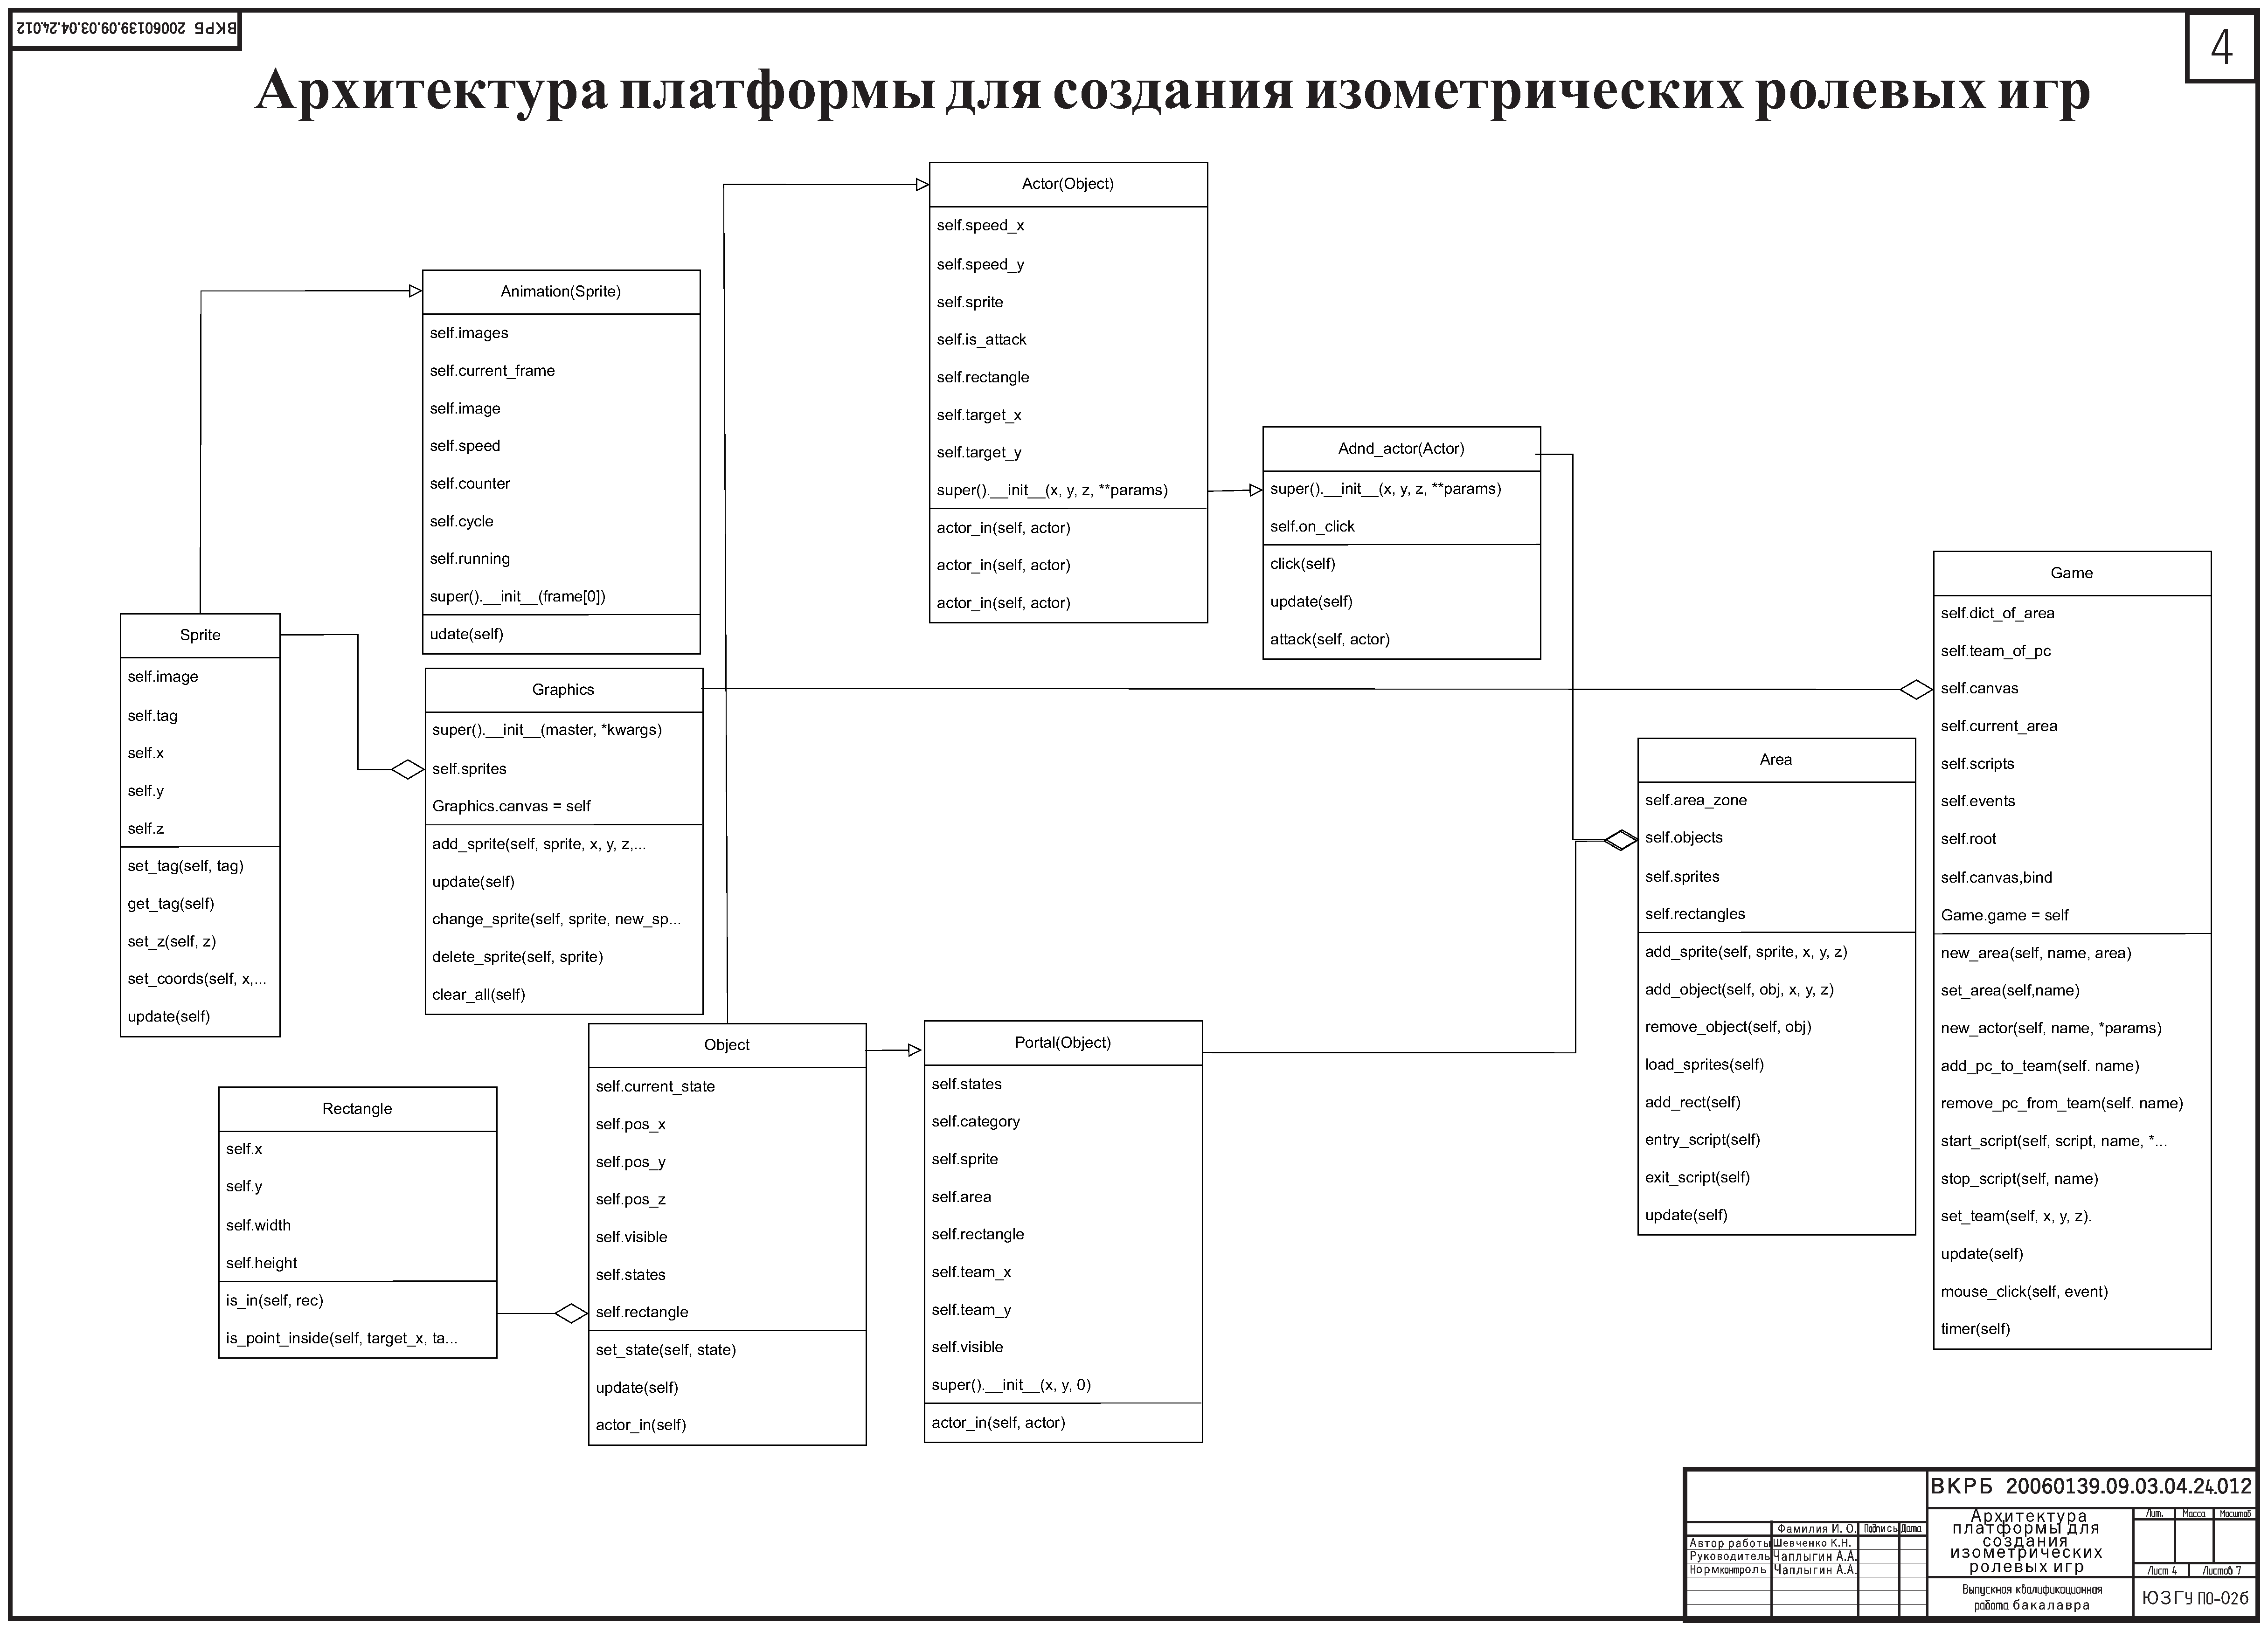
\includegraphics[width=0.82\linewidth]{плакат_4.esp}
	\заголовок{Диаграмма классов}
	\label{плакат_4.esp:image}      
\end{плакат}

\begin{плакат}
	
\includegraphics[width=0.82\linewidth]{плакат_5.esp}
	\заголовок{Модель работы сценариев}
	\label{плакат_5.esp:image}      
\end{плакат}

\begin{плакат}
	
\includegraphics[width=0.82\linewidth]{плакат_6.esp}
	\заголовок{Модульное тестирование платформы}
	\label{плакат_6.esp:image}      
\end{плакат}

\begin{плакат}
	
\includegraphics[width=0.82\linewidth]{плакат_7.esp}
	\заголовок{Заключение}
	\label{плакат_7.esp:image}      
\end{плакат}

\end{landscape}
}\fi
\ifПрактика{}\else{\appendix{Фрагменты исходного кода программы}

sprite.py
\lstinputlisting[language=Python, frame=none]{sprite.py}

graphics.py
\lstinputlisting[language=Python, frame=none]{graphics.py}

game.py
\lstinputlisting[language=Python, frame=none]{game.py}

\ifВКР{
\newpage
\addcontentsline{toc}{section}{На отдельных листах (CD-RW в прикрепленном конверте)}
\begin{center}
\textbf{Место для диска}
\end{center}
}\fi
}\fi
\end{document}
